%%% Hlavní soubor. Zde se definují základní parametry a odkazuje se na ostatní části. %%%

%% Verze pro jednostranný tisk:
% Okraje: levý 40mm, pravý 25mm, horní a dolní 25mm
% (ale pozor, LaTeX si sám přidává 1in)
\documentclass[12pt,a4paper]{report}
\setlength\textwidth{145mm}
\setlength\textheight{247mm}
\setlength\oddsidemargin{15mm}
\setlength\evensidemargin{15mm}
\setlength\topmargin{0mm}
\setlength\headsep{0mm}
\setlength\headheight{0mm}
% \openright zařídí, aby následující text začínal na pravé straně knihy
\let\openright=\clearpage

%% Pokud tiskneme oboustranně:
% \documentclass[12pt,a4paper,twoside,openright]{report}
% \setlength\textwidth{145mm}
% \setlength\textheight{247mm}
% \setlength\oddsidemargin{14.2mm}
% \setlength\evensidemargin{0mm}
% \setlength\topmargin{0mm}
% \setlength\headsep{0mm}
% \setlength\headheight{0mm}
% \let\openright=\cleardoublepage

%% Vytváříme PDF/A-2u
\usepackage[a-2u]{pdfx}

%% Přepneme na českou sazbu a fonty Latin Modern
\usepackage[czech]{babel}
\usepackage{lmodern}
\usepackage[T1]{fontenc}
\usepackage{textcomp}

%% Použité kódování znaků: obvykle latin2, cp1250 nebo utf8:
\usepackage[utf8]{inputenc}

%%% Další užitečné balíčky (jsou součástí běžných distribucí LaTeXu)
\usepackage{amsmath}        % rozšíření pro sazbu matematiky
\usepackage{amsfonts}       % matematické fonty
\usepackage{amsthm}         % sazba vět, definic apod.
\usepackage{bbding}         % balíček s nejrůznějšími symboly
% (čtverečky, hvězdičky, tužtičky, nůžtičky, ...)
\usepackage{bm}             % tučné symboly (příkaz \bm)
\usepackage{graphicx}       % vkládání obrázků
\usepackage{fancyvrb}       % vylepšené prostředí pro strojové písmo
\usepackage{indentfirst}    % zavede odsazení 1. odstavce kapitoly
\usepackage{natbib}         % zajištuje možnost odkazovat na literaturu
% stylem AUTOR (ROK), resp. AUTOR [ČÍSLO]
\usepackage[nottoc]{tocbibind} % zajistí přidání seznamu literatury,
% obrázků a tabulek do obsahu
\usepackage{icomma}         % inteligetní čárka v matematickém módu
\usepackage{dcolumn}        % lepší zarovnání sloupců v tabulkách
\usepackage{booktabs}       % lepší vodorovné linky v tabulkách
\usepackage{paralist}       % lepší enumerate a itemize
\usepackage{xcolor}
\usepackage{hyperref}         % barevná sazba

%%% Údaje o práci

% Název práce v jazyce práce (přesně podle zadání)
\newcommand{\NazevPrace}{Autonomní křižovatka}

% Název práce v angličtině
\newcommand{\NazevPraceEN}{Autonomous traffic junction}

% Jméno autora
\newcommand{\AutorPrace}{Jiří Kotal}

% Rok odevzdání
\newcommand{\RokOdevzdani}{2022}

% Název katedry nebo ústavu, kde byla práce oficiálně zadána
% (dle Organizační struktury MFF UK, případně plný název pracoviště mimo MFF)
\newcommand{\Katedra}{Katedra teoretické informatiky a matematické logiky}
\newcommand{\KatedraEN}{Department of Theoretical Computer Science and Mathematical Logic}

% Jedná se o katedru (department) nebo o ústav (institute)?
\newcommand{\TypPracoviste}{Katedra}
\newcommand{\TypPracovisteEN}{Department}

% Vedoucí práce: Jméno a příjmení s~tituly
\newcommand{\Vedouci}{prof. RNDr. Roman Barták, Ph.D.}

% Pracoviště vedoucího (opět dle Organizační struktury MFF)
\newcommand{\KatedraVedouciho}{Katedra teoretické informatiky a matematické logiky}
\newcommand{\KatedraVedoucihoEN}{Department of Theoretical Computer Science and Mathematical Logic}

% Studijní program a obor
\newcommand{\StudijniProgram}{Informatika}
\newcommand{\StudijniObor}{Obecná informatika}

% Nepovinné poděkování (vedoucímu práce, konzultantovi, tomu, kdo
% zapůjčil software, literaturu apod.)
\newcommand{\Podekovani}{%
	Poděkování.
}

% Abstrakt (doporučený rozsah cca 80-200 slov; nejedná se o zadání práce)
\newcommand{\Abstrakt}{
	Práce se zabývá problematikou průjezdů vozů plně automatizovanou křižovatkou
	a~to z~pohledu multi-agentního hledání cest (MAPF, multi-agent path finding).
	Cílem je prozkoumat různé abstrakce křižovatky a různé přístupy pro~hledání nekolizního průjezdu křižovatkou.
	Zkoumané techniky jsou implementovány a empiricky porovnány v~simulovaném prostředí.
}

\newcommand{\AbstraktEN}{
	This~work deals with the~problem of cars transiting through an~autonomous traffic junction
	from~the~perspective of~multi-agent path finding (MAPF).
	The~aim is to~explore different abstractions of~the~junction
	and different approaches to~find collision-free trajectories through the~junction.
	Various techniques are implemented and empirically compared in~a~simulated environment.
}


% 3 až 5 klíčových slov (doporučeno), každé uzavřeno ve složených závorkách
\newcommand{\KlicovaSlova}{%
		{plánování cest}
		{koordinace}
		{multi-agentní systémy}
		{křižovatka}
		{doprava}
}
\newcommand{\KlicovaSlovaEN}{%
		{path planning}
		{coordination}
		{multi-agent systems}
		{traffic junction}
		{transport}
}

%% Balíček hyperref, kterým jdou vyrábět klikací odkazy v PDF,
%% ale hlavně ho používáme k uložení metadat do PDF (včetně obsahu).
%% Většinu nastavítek přednastaví balíček pdfx.
\hypersetup{unicode}
\hypersetup{breaklinks=true}

%% Definice různých užitečných maker (viz popis uvnitř souboru)
%%% Tento soubor obsahuje definice různých užitečných maker a prostředí %%%
%%% Další makra připisujte sem, ať nepřekáží v ostatních souborech.     %%%

%%% Drobné úpravy stylu

% Tato makra přesvědčují mírně ošklivým trikem LaTeX, aby hlavičky kapitol
% sázel příčetněji a nevynechával nad nimi spoustu místa. Směle ignorujte.
\makeatletter
\def\@makechapterhead#1{
  {\parindent \z@ \raggedright \normalfont
   \Huge\bfseries \thechapter. #1
   \par\nobreak
   \vskip 20\p@
}}
\def\@makeschapterhead#1{
  {\parindent \z@ \raggedright \normalfont
   \Huge\bfseries #1
   \par\nobreak
   \vskip 20\p@
}}
\makeatother

% Toto makro definuje kapitolu, která není očíslovaná, ale je uvedena v obsahu.
\def\chapwithtoc#1{
\chapter*{#1}
\addcontentsline{toc}{chapter}{#1}
}

% Trochu volnější nastavení dělení slov, než je default.
\lefthyphenmin=2
\righthyphenmin=2

% Zapne černé "slimáky" na koncích řádků, které přetekly, abychom si
% jich lépe všimli.
\overfullrule=1mm

%%% Makra pro definice, věty, tvrzení, příklady, ... (vyžaduje baliček amsthm)

\theoremstyle{plain}
\newtheorem{veta}{Věta}
\newtheorem{lemma}[veta]{Lemma}
\newtheorem{tvrz}[veta]{Tvrzení}

\theoremstyle{plain}
\newtheorem{definice}{Definice}

\theoremstyle{remark}
\newtheorem*{dusl}{Důsledek}
\newtheorem*{pozn}{Poznámka}
\newtheorem*{prikl}{Příklad}

%%% Prostředí pro důkazy

\newenvironment{dukaz}{
  \par\medskip\noindent
  \textit{Důkaz}.
}{
\newline
\rightline{$\qedsymbol$}
}

%%% Prostředí pro sazbu kódu, případně vstupu/výstupu počítačových
%%% programů. (Vyžaduje balíček fancyvrb -- fancy verbatim.)

\DefineVerbatimEnvironment{code}{Verbatim}{fontsize=\small, frame=single}

%%% Prostor reálných, resp. přirozených čísel
\newcommand{\R}{\mathbb{R}}
\newcommand{\N}{\mathbb{N}}

%%% Užitečné operátory pro statistiku a pravděpodobnost
\DeclareMathOperator{\pr}{\textsf{P}}
\DeclareMathOperator{\E}{\textsf{E}\,}
\DeclareMathOperator{\var}{\textrm{var}}
\DeclareMathOperator{\sd}{\textrm{sd}}

%%% Příkaz pro transpozici vektoru/matice
\newcommand{\T}[1]{#1^\top}

%%% Vychytávky pro matematiku
\newcommand{\goto}{\rightarrow}
\newcommand{\gotop}{\stackrel{P}{\longrightarrow}}
\newcommand{\maon}[1]{o(n^{#1})}
\newcommand{\abs}[1]{\left|{#1}\right|}
\newcommand{\dint}{\int_0^\tau\!\!\int_0^\tau}
\newcommand{\isqr}[1]{\frac{1}{\sqrt{#1}}}

%%% Vychytávky pro tabulky
\newcommand{\pulrad}[1]{\raisebox{1.5ex}[0pt]{#1}}
\newcommand{\mc}[1]{\multicolumn{1}{c}{#1}}


%% Titulní strana a různé povinné informační strany
\begin{document}
	%%% Titulní strana práce a další povinné informační strany

%%% Titulní strana práce

\pagestyle{empty}
\hypersetup{pageanchor=false}

\begin{center}

	\centerline{\mbox{
\includegraphics[width=166mm]{../img/logo-cs}}}

	\vspace{-8mm}
	\vfill

	{\textbf{\Large BAKALÁŘSKÁ PRÁCE}}

	\vfill

	{\LARGE\AutorPrace}

	\vspace{15mm}

	{\LARGE\bfseries\NazevPrace}

	\vfill

	\Katedra

	\vfill

	{
		\centerline{\vbox{\halign{\hbox to 0.45\hsize{\hfil #}&\hskip 0.5em\parbox[t]{0.45\hsize}{\raggedright #}\cr
		Vedoucí bakalářské práce:&\Vedouci \cr
		\noalign{\vspace{2mm}}
		Studijní program:&\StudijniProgram \cr
		\noalign{\vspace{2mm}}
		Studijní obor:&\StudijniObor \cr
		}}}}

	\vfill

% Zde doplňte rok
	Praha \RokOdevzdani

\end{center}

\newpage

%%% Následuje vevázaný list -- kopie podepsaného "Zadání bakalářské práce".
%%% Toto zadání NENÍ součástí elektronické verze práce, nescanovat.

%%% Strana s čestným prohlášením k bakalářské práci

\openright
\hypersetup{pageanchor=true}
\pagestyle{plain}
\pagenumbering{roman}
\vglue 0pt plus 1fill

\noindent
Prohlašuji, že jsem tuto bakalářskou práci vypracoval(a) samostatně a výhradně
s~použitím citovaných pramenů, literatury a dalších odborných zdrojů.
Tato práce nebyla využita k získání jiného nebo stejného titulu.

\medskip\noindent
Beru na~vědomí, že se na moji práci vztahují práva a povinnosti vyplývající
ze zákona č. 121/2000 Sb., autorského zákona v~platném znění, zejména skutečnost,
že Univerzita Karlova má právo na~uzavření licenční smlouvy o~užití této
práce jako školního díla podle §60 odst. 1 autorského zákona.

\vspace{10mm}

\hbox{\hbox to 0.5\hsize{%
	V \hbox to 6em{\dotfill} dne \hbox to 6em{\dotfill}
	\hss}\hbox to 0.5\hsize{\dotfill\quad}}
\smallskip
\hbox{\hbox to 0.5\hsize{}\hbox to 0.5\hsize{\hfil Podpis autora\hfil}}

\vspace{20mm}
\newpage

%%% Poděkování

\openright

\noindent
\Podekovani

\newpage

%%% Povinná informační strana bakalářské práce

\openright

\vbox to 0.5\vsize{
	\setlength\parindent{0mm}
	\setlength\parskip{5mm}

	Název práce:
	\NazevPrace

	Autor:
	\AutorPrace

	\TypPracoviste:
	\Katedra

	Vedoucí bakalářské práce:
	\Vedouci, \KatedraVedouciho

	Abstrakt:
	\Abstrakt

	Klíčová slova:
	\KlicovaSlova

	\vss}\nobreak\vbox to 0.49\vsize{
	\setlength\parindent{0mm}
	\setlength\parskip{5mm}

	Title:
	\NazevPraceEN

	Author:
	\AutorPrace

	\TypPracovisteEN:
	\KatedraEN

	Supervisor:
	\Vedouci, \KatedraVedoucihoEN

	Abstract:
	\AbstraktEN

	Keywords:
	\KlicovaSlovaEN

	\vss}

\newpage

\openright
\pagestyle{plain}
\pagenumbering{arabic}
\setcounter{page}{1}


%%% Strana s automaticky generovaným obsahem bakalářské práce

	\tableofcontents

%%% Jednotlivé kapitoly práce jsou pro přehlednost uloženy v samostatných souborech
	\chapter*{Úvod}\label{ch:uvod}
\addcontentsline{toc}{chapter}{Úvod}

Vývoj aut jde velice rychle kupředu.
Svět s~autonomními auty, které budou řídit za~nás, je v~dnešní době představitelný.
Samořiditelná auta už~jezdí mezi námi, avšak stále jsou značně omezeny manuálně řízenými vozy a~zákony.
Tato auta mají téměř okamžitou odezvu na~vnější vlivy, dokáží se navigovat skrze dopravu s~vysokou přesností a~také mají výhodu jednodušší vzájemné komunikace.
Těchto vlastností se dá využít pro~zvýšení efektivity dopravní sítě.
Zlepšení na~běžných silnicích nemusí být značné, avšak u~křižovatek by~mohl být rozdíl velmi velký.

Zaměřit se na~křižovatky je důležité i~z~pohledu nehodovosti.
Ačkoliv většina silniční komunikace probíhá na~nekřížících se úsecích, na~našem území dochází kolem $21\%$ všech nehod
právě na~křižovatkách (\href{https://www.czso.cz/documents/10180/20534694/32025414a06.pdf}{Český Statistický Úřad}).

Tato práce se~zabývá problémem projetí co~největšího množství autonomních aut skrze křižovatku.
K~řešení tohoto problému používá křižovatka určitou centrální skříňku, se kterou auta komunikují.
Po~příjezdu auta auto nahlásí křižovatce odkud přijíždí a kam by chtělo jet.
Křižovatka poté autu naplánuje nekolizní trasu skrze křižovatku.

Simulovaný svět obsahuje značná zjednodušení reálného světa, avšak dle~mého názoru jsou nápady určitou formou přenositelné.
Práce obsahuje různá řešení tohoto problému pomocí simulovaného prostředí na~různých křižovatkách a~množství aut.
Tato~řešení jsou následně porovnána dle~rozličných parametrů.


\section{Abstraktní model křižovatky}\label{sec:krizovatka}

%Shrnutí hledání na grafu, definice grafu.
%
%Popis různých vzhledů křižovatky.
%Převod křižovatky na graf a parametry převodu.


Všechny mnou používané algoritmy jsou založeny na~prohledávání orientovaného grafu.
Z~tohoto důvodu je nutné převést křižovatku na~graf.
Převod je proveden rozdělením křižovatky na~diskrétní nepřekrývající~se bloky zaplňující celou plochu křižovatky.
Mezi sousedními bloky mohou auta přejíždět.

Formálně je křižovatka převedena na~orientovaný graf,
kde~každý blok je reprezentován jedním vrcholem a hrany vedou mezi bloky se společnou stěnou.
%Vzdálenost mezi sousedními bloky (čas přejezdu) je u~všech bloků stejný a trvá právě jeden krok simulace.  TODO

Bloky jsou rozděleny do~třech skupin.
První skupina jsou vrcholy reprezentující vnitřní plochu křižovatky.
Zbylé dvě skupiny reprezentují \hyperref[par:vjezdy]{vjezdy do~křižovatky} a \hyperref[par:vyjezdy]{výjezdy z~křižovatky}.

Rozhodl jsem se pro~$3$~různé typy křižovatek určené rozdělením plochy na~bloky.
Tyto~typy budu nazývat \hyperref[subsec:ctvercovy_typ]{čtvercový}, \hyperref[subsec:oktagonalni_typ]{oktagonální}
a~\hyperref[subsec:hexagonalni_typ]{hexagonální}.

Rozdělení křižovatky má určité parametry ovlivňující výsledný graf.
Těmito parametry jsou \hyperref[par:velikost_krizovatky]{velikost křižovatky},
\hyperref[par:vjezdy]{počet vjezdů} a~\hyperref[par:vyjezdy]{počet výjezdů}.

\paragraph{Velikost křižovatky}\label{par:velikost_krizovatky} značí z~kolika bloků se křižovatka skládá.
Obecně je hodnota \hyperref[par:velikost_krizovatky]{velikosti křižovatky} rovna počtu bloků na jedné hraně křižovatky.
Přesný význam je popsán zvlášť v~jednotlivých kapitolách.
Na~\hyperref[par:velikost_krizovatky]{velikosti křižovatky} závisí tzv.~\hyperref[par:velikost_bloku]{velikost bloku}.

\paragraph{Velikost bloku}\label{par:velikost_bloku} značí velikost základních bloků rozdělení
(odpovídá vzdálenosti mezi vrcholy), opět se ale u~různých typů liší.
Tuto~veličinu zavádím kvůli jednoduchému porovnání velikosti auta vůči bloku.

Každý typ křižovatky má předurčený počet \emph{směrů}, ze~kterých auta přijíždějí.

\paragraph{Vjezdy}\label{par:vjezdy} značí množství vrcholů reprezentujících pruhy vjezdů z~každého \emph{směru} křižovatky.
Tyto vrcholy mají pouze jednu výstupní hranu a žádná hrana do nich nevede.

\paragraph{Výjezdy}\label{par:vyjezdy} mají podobný význam, určují počet výjezdních pruhů z~každého \emph{směru}.
Vrcholy výjezdů mají oproti \hyperref[par:vjezdy]{vjezdům} jednu vstupní hranu a žádnou výstupní.

Jelikož se na~silnicích auta pohybují po~pravé straně silnice,
jsou vjezdy a výjezdy z~jednoho směru seřazeny vůči hraně křižovatky zleva doprava v~pořadí
\ref{str:mezera_l}, \hyperref[par:vyjezdy]{výjezdy}, \ref{str:mezera_s}, \hyperref[par:vyjezdy]{vjezdy}, \ref{str:mezera_p}.
Kde~\emph{mezeraL}\labeltext{mezeraL}{str:mezera_l}, \emph{mezeraS}\labeltext{mezeraS}{str:mezera_s}
a~\emph{mezeraP}\labeltext{mezeraP}{str:mezera_p} značí posloupnost vrcholů na~hraně křižovatky
nesousedících s~vjezdem ani~výjezdem.
Všechny \hyperref[par:vjezdy]{vjezdy} jsou vždy přímo vedle sebe a \hyperref[par:vyjezdy]{výjezdy} taktéž.
Většina křižovatek je symetrická proto jsem určil, že velikost části \ref{str:mezera_l} bude shodná s~velikostí části \ref{str:mezera_p}.
Opět kvůli symetričnosti jsem zvolil velikost části \ref{str:mezera_p} co~nejblíže velikostem
krajových mezer \ref{str:mezera_l} a \ref{str:mezera_p}.
Platí tedy $\ref{str:mezera_l}=\ref{str:mezera_p}\wedge(\ref{str:mezera_s}=\ref{str:mezera_l}\vee\ref{str:mezera_s}+1=\ref{str:mezera_l})$.

\hyperref[par:pruh]{Pruhy} jsou známý koncept u křižovatek a v dopravě obecně.
Rozhodl jsem se proto formálně definovat \hyperref[par:pruh]{pruh}.

\paragraph{Pruh}\label{par:pruh} mezi určitým vjezdem a výjezdem definuji jako nejkratší cestu mezi těmito vrcholy.
Délka cesty je určena počtem vrcholů, přes které vede.
Pokud vedou dvě různé cesty přes stejný počet vrcholů, je upřednostněna ta, na~které musí auto méně zatáčet.
Čili cesty jsou následně porovnány podle úhlu, o~který se musí auta během jízdy otočit.
Pokud je i~tato hodnota stejná, porovnávají se auta podle počtu vrcholů, kterými neprojíždí rovně.
Při~posledním porovnání je preferována cesta s~více vrcholy.
Takto jsem se rozhodl, protože díky tomu budou mít auta méně ostré zatáčky.

\subsection{Čtvercový typ}\label{subsec:ctvercovy_typ}

\nameref{subsec:ctvercovy_typ} křižovatky rozděluje plochu do~čtvercových bloků.
Celková hlavní plocha křižovatky (tedy veškerá plocha mimo
\hyperref[par:vjezdy]{vjezdy} a \hyperref[par:vyjezdy]{výjezdy}) tvoří čtverec.

\nameref{par:velikost_krizovatky} značí počet bloků na~jedné straně plochy křižovatky.
Celkový počet bloků hlavní plochy křižovatky tudíž činí $g^2$,
kde $g$ je \hyperref[par:velikost_krizovatky]{velikost křižovatky}.
Pozice vrcholu je přesně uprostřed jemu odpovídajícího bloku.
Mezi každými bloky, který spolu sdílí stěnu, vede ve~výsledným grafu hrana.
Tento typ křižovatky má čtyři směry, jeden směr na~každé straně čtverce hlavní plochy.
Křižovatka je převedena na~graf s~$g^2 + 4i + 4o$ vrcholy,
kde $g$ opět značí \hyperref[par:velikost_krizovatky]{velikost},
$i$~\hyperref[par:vjezdy]{vjezdy} a $o$~\hyperref[par:vyjezdy]{výjezdy}.

Ukázka křižovatky s~\hyperref[par:velikost_krizovatky]{velikostí}~$4$, jedním \hyperref[par:vjezdy]{vjezdem} a
jedním \hyperref[par:vyjezdy]{výjezdem} je vidět na~obrázku~\ref{fig:square_type_graph}.
Na~obrázku jsou šedou barvou označeny vrcholy značící běžnou plochu křižovatky,
červeno-šedou barvou označeny vrcholy reprezentující \hyperref[par:vjezdy]{vjezdy} a
modro-šedé vrcholy reprezentují \hyperref[par:vyjezdy]{výjezdy}.

\begin{figure}[h]
	\centering
	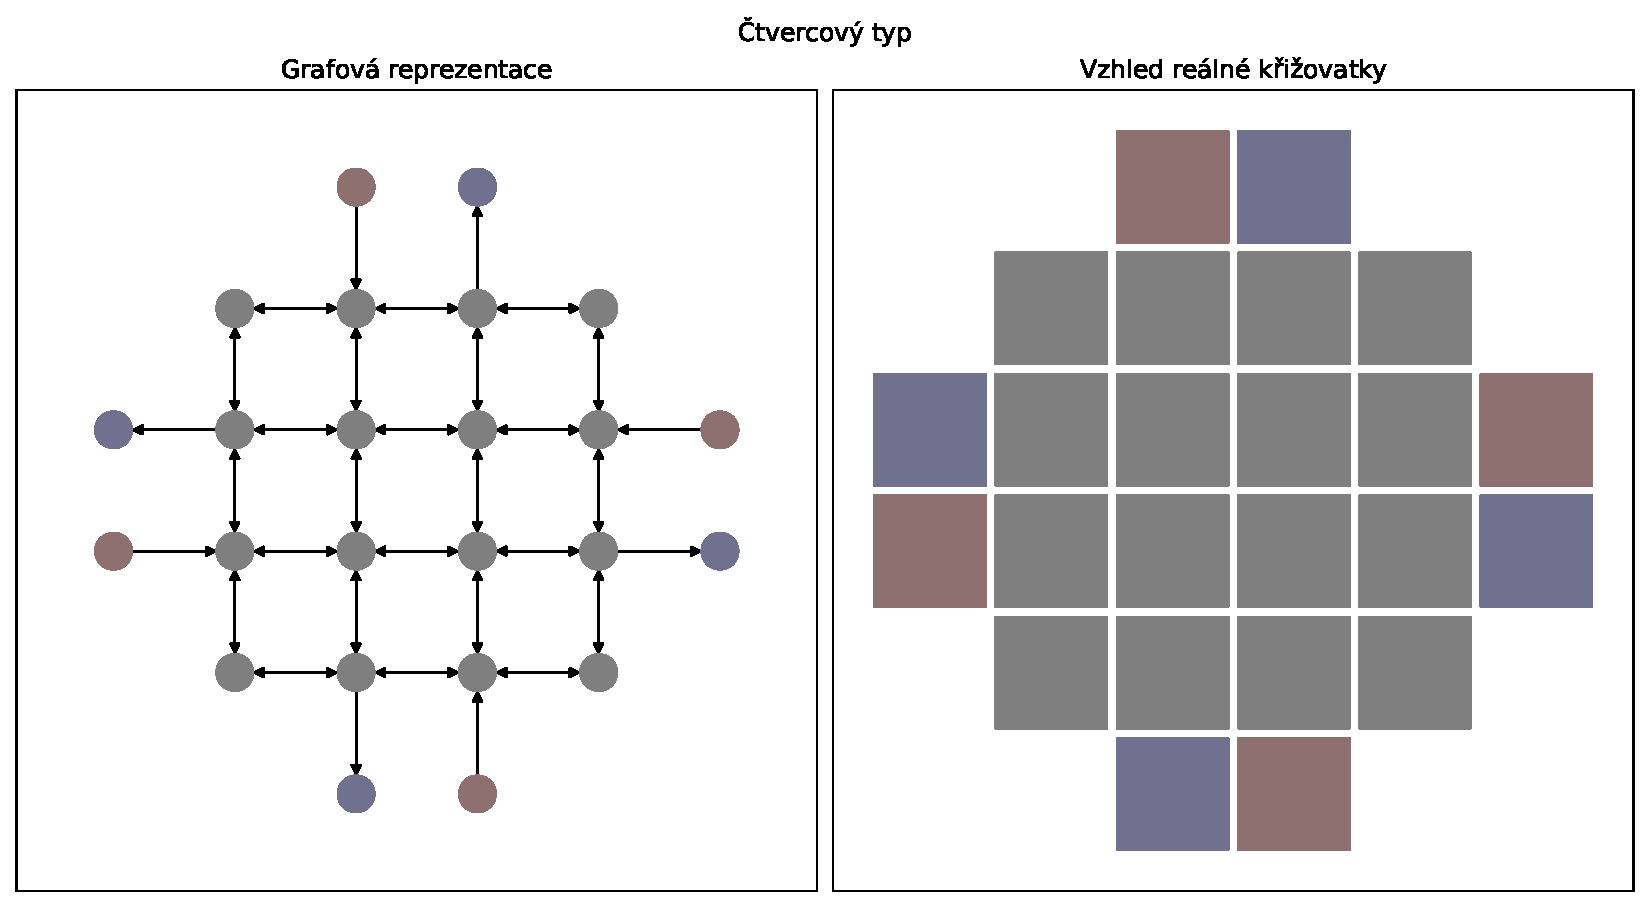
\includegraphics[width=\textwidth]{../img/Square_grid}
	\caption{Ukázka čtvercového typu křižovatky.}
	\label{fig:square_type_graph}
\end{figure}

\subsection{Oktagonální typ}\label{subsec:oktagonalni_typ}

\nameref{subsec:oktagonalni_typ} křižovatky vychází z~typu \hyperref[subsec:ctvercovy_typ]{čtvercového},
avšak rozšiřuje tento typ o~možnost diagonální jízdy.
Tohoto efektu docílí křižovatka přidáním dodatečných vrcholů mezi každé čtvercové bloky dotýkající se rohem.
Z~vizuálního hlediska se ze~čtvercových bloků stanou oktagonální (osmiúhelníkové),
odtud plyne samostatný název tohoto typu.
Tyto bloky mohou mít až~$8$~sousedů.
Mezi těmito oktagonálními bloky vzniknou nové bloky reprezentující diagonální přejezdy.
Nově vytvořené bloky mají nanejvýše $4$~sousedy, a tvoří pomyslný čtverec.
Z~vizuálních důvodů byly odebrány rohové bloky.

\nameref{par:velikost_krizovatky}, \hyperref[par:vjezdy]{vjezdy} a \hyperref[par:vyjezdy]{výjezdy}
mají stejný význam jako u~\hyperref[subsec:ctvercovy_typ]{čtvercového typu}.
Počet vrcholů u~této křižovatky činí $g^2 - 4 + (g-1)^2 + 4i + 4o = 2g^2 - 2g - 3 + 4(i + o)$,
kde $g$ je \hyperref[par:velikost_krizovatky]{velikost},
$i$ počet \hyperref[par:vjezdy]{vjezdů} a $o$ počet \hyperref[par:vyjezdy]{výjezdů}.
\nameref{par:velikost_bloku} je vzdálenost mezi dvěma sousedními vrcholy reprezentujícími oktagonální blok,
opět totožná s~velikostí bloku u~čtvercového typu.

Na~obrázku (Obrázek~\ref{fig:octagonal_type_graph}) je znázorněn příklad
\hyperref[subsec:oktagonali_typ]{oktagonálního typu} křižovatky s~\hyperref[par:velikost_krizovatky]{velikostí}~$4$,
jedním \hyperref[par:vjezdy]{vjezdem} a jedním \hyperref[par:vyjezdy]{výjezdem}.

Barvy vrcholů a bloků jsou stejné jako u~\hyperref[subsec:ctvercovy_typ]{čtvercového typu},
šedou barvou jsou označeny vrcholy značící běžnou plochu křižovatky,
červeno-šedou barvou označeny vrcholy reprezentující \hyperref[par:vjezdy]{vjezdy} a
modro-šedé vrcholy reprezentují \hyperref[par:vyjezdy]{výjezdy}.

\begin{figure}[h]
	\centering
	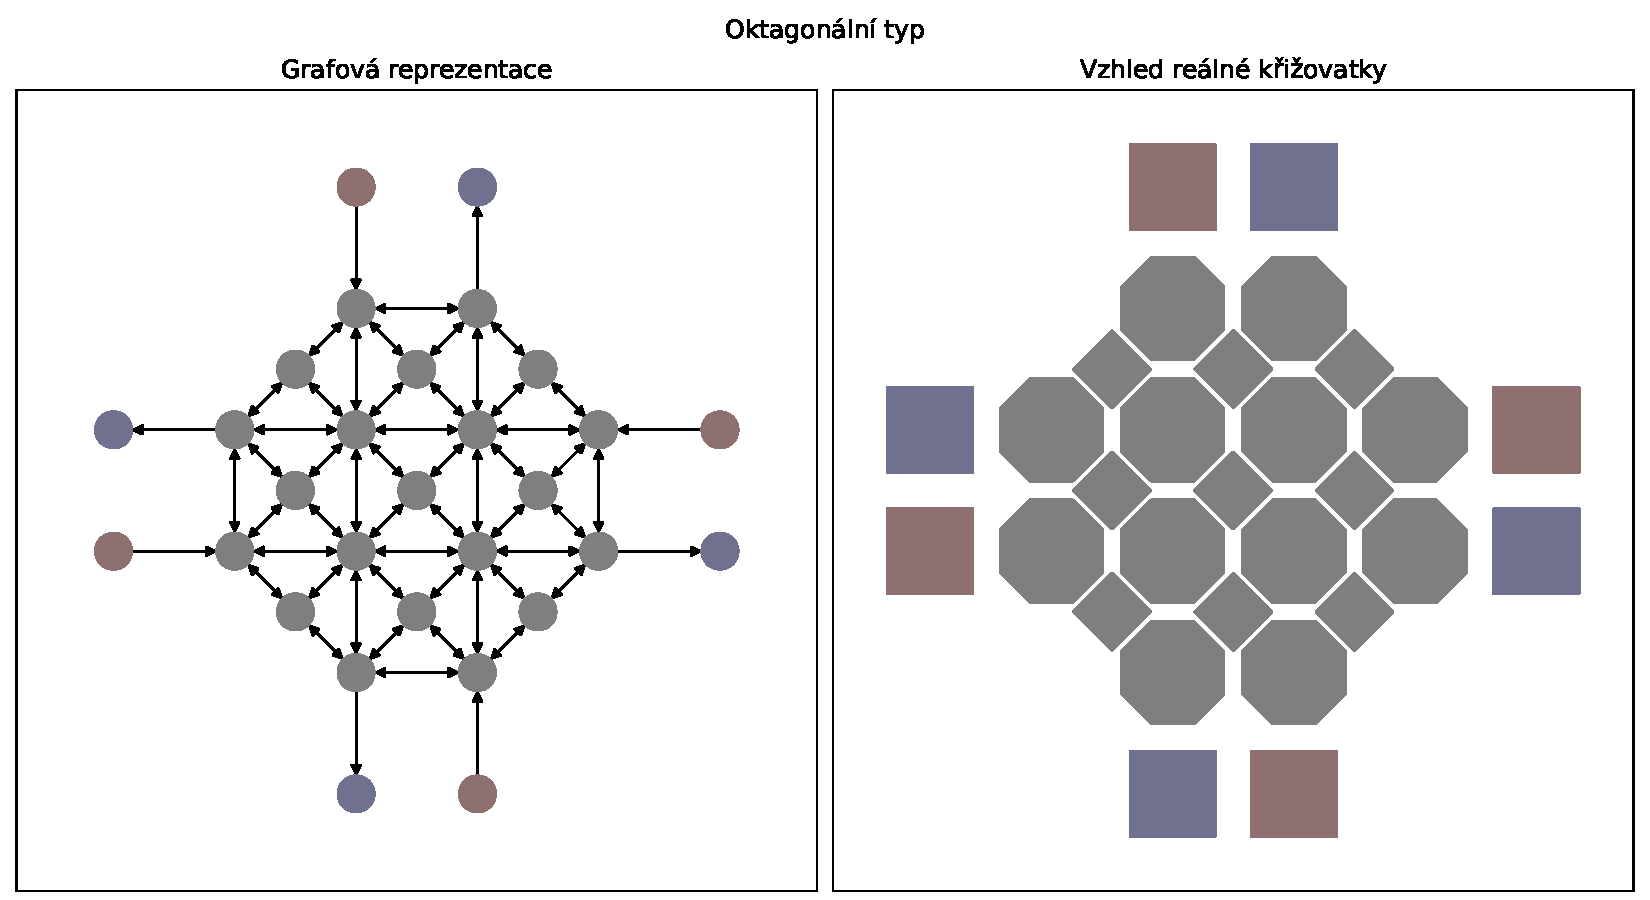
\includegraphics[width=\textwidth]{../img/Octagonal_grid}
	\caption{Ukázka oktagonálního typu křižovatky.}
	\label{fig:octagonal_type_graph}
\end{figure}

\subsection{Hexagonální typ}\label{subsec:hexagonalni_typ}

\nameref{subsec:hexagonalni_typ} je tvořen bloky s~tvary hexagonu (šestiúhelníku).
Při~převodu křižovatky na~graf je každý hexagonální blok nahrazen jedním vrcholem ležícím uprostřed původního bloku.
Opět hrany grafu vedou mezi bloky se společnou stěnou.
Každý blok má tedy až~$6$~sousedů.
Tyto bloky tvoří dohromady plochu tvaru velkého hexagonu.
Díky této reprezentaci má křižovatka tohoto typu $6$~směrů odkud mohou auta přijíždět.

Toto rozdělení sebou nese jednu velkou nevýhodu.
Pokud chce auto jet rovně skrze křižovatku (do~protilehlého směru), křižovatka mu nemůže nabídnout rovnou cestu.

\nameref{par:velikost_krizovatky} u~tohoto typu opět značí počet bloků na~jedné straně celkové plochy.
Hodnota je taktéž rovna počtu vrcholů z~kraje křižovatky do~středu.
Počet vrcholů grafu tedy činí $6 \times g \times (g-1) + 6i + 6o$,
kde $g$ je \hyperref[par:velikost_krizovatky]{velikost},
$i$ počet \hyperref[par:vjezdy]{vjezdů} a $o$ počet \hyperref[par:vyjezdy]{výjezdů}.
\nameref{par:velikost_bloku} je opět vzdálenost mezi dvěma sousedními vrcholy.

Na~obrázku (Obrázek~\ref{fig:hexagonal_type_graph}) je znázorněn příklad
\hyperref[subsec:hexagonalni_typ]{hexagonálního typu} křižovatky s~\hyperref[par:velikost_krizovatky]{velikostí}~$4$,
jedním \hyperref[par:vjezdy]{vjezdem} a jedním \hyperref[par:vyjezdy]{výjezdem}.

Barvy vrcholů a bloků jsou opět stejné.
Šedou barvou jsou označeny vrcholy značící běžnou plochu křižovatky,
červeno-šedou barvou označeny vrcholy reprezentující \hyperref[par:vjezdy]{vjezdy} a
modro-šedé vrcholy reprezentují \hyperref[par:vyjezdy]{výjezdy}.

\begin{figure}[h]
	\centering
	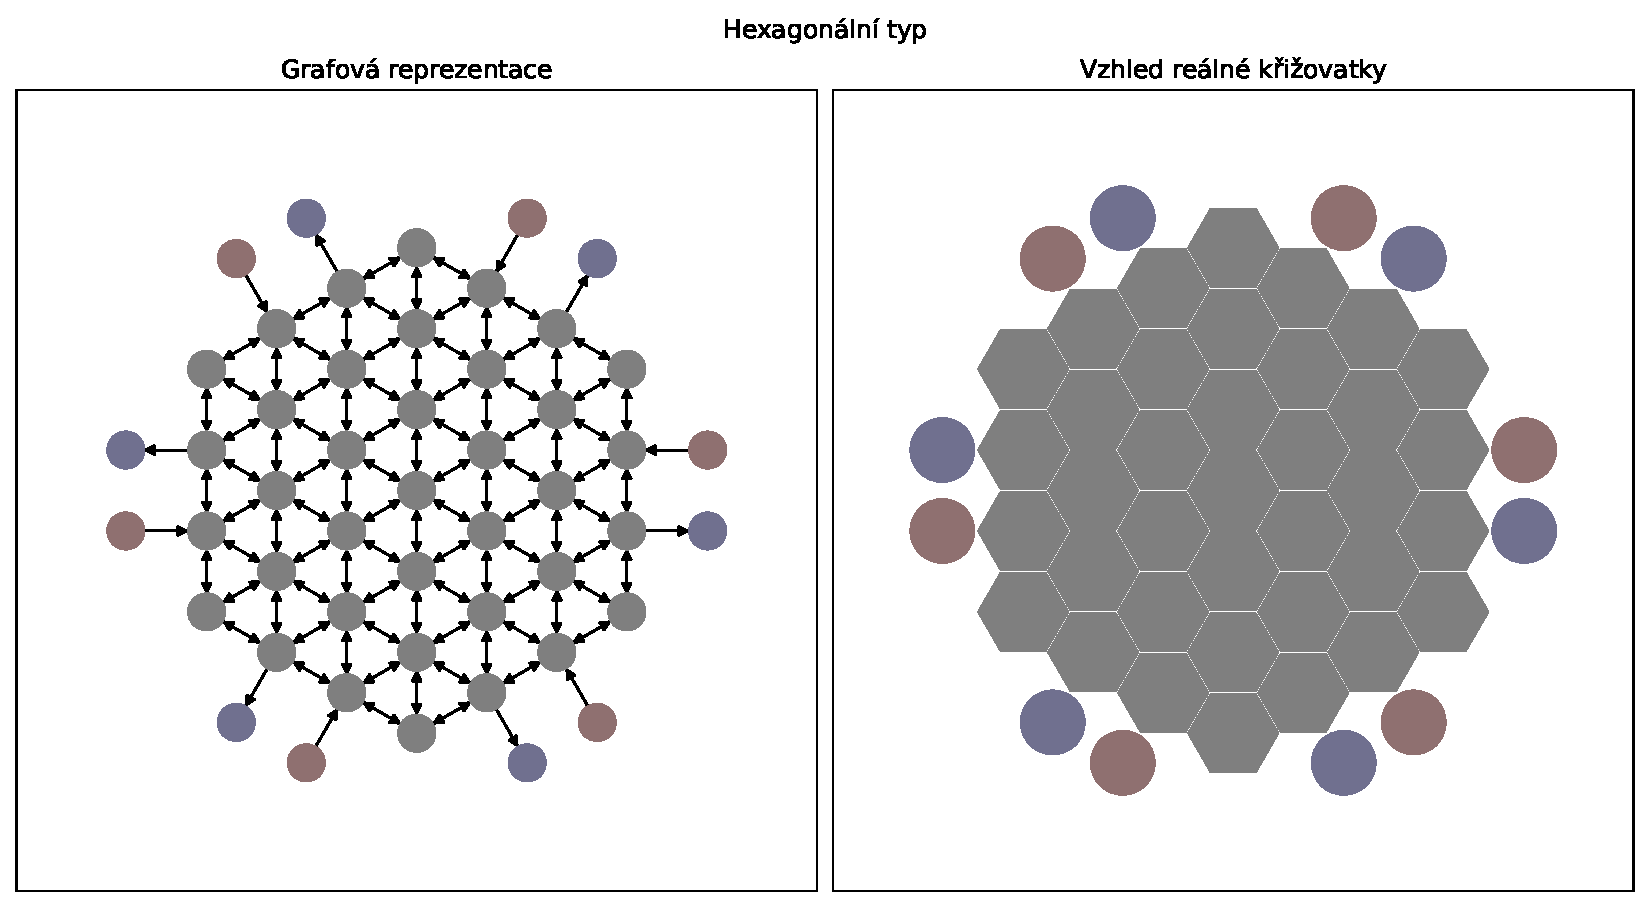
\includegraphics[width=\textwidth]{../img/Hexagonal_grid}
	\caption{Ukázka hexagonálního typu křižovatky.}
	\label{fig:hexagonal_type_graph}
\end{figure}


\section{Agent}\label{sec:agent}

%Popis zjednodušení auta na agenta.
%Popis parametrů agenta.


\nameref{sec:agent} je zjednodušení chytrého auta pro snadnější použití v~algoritmech.
Tvar \hyperref[sec:agent]{agenta} je zjednodušený na~obdélník, který má určitou délku, šířku a naklonění v~rovině.
Tento obdélník reprezentuje pohled na~auto shora.
Šířka a délka \hyperref[sec:agent]{agenta} je určená vůči \hyperref[par:velikost_bloku]{velikosti bloku} dané křižovatky.

Pokud se nějaké dva obdélníky protnou, nastane srážka příslušných dvou \hyperref[sec:agent]{agentů}.
\hyperref[sec:agent]{Agenti} nemají žádný způsob jak informovat křižovatku o~srážce.
Z~toho důvodu po~kolizi sražení \hyperref[sec:agent]{agenti} zmizí a žádní jiní \hyperref[sec:agent]{agenti} s~nimi nemohou kolidovat.

Jelikož se \hyperref[sec:agent]{agent} pohybuje po~hranách grafu křižovatky, je jeho cesta složená z~úseček.
Proto jsem umožnil \hyperref[sec:agent]{agentovy} otáčet se na~místě a otáčení probíhá okamžitě po~příjezdu do~vrcholu.
\hyperref[sec:agent]{Agent} tedy pořád cestuje a otáčí se vždy ve~směru jízdy.
Tato vlastnost by neměla mít na~pohyb auta velký vliv, pokud je auto dostatečně malé
oproti vzdálenostem vrcholů grafu křižovatky (\hyperref[par:velikost_bloku]{velikosti bloku}).

\hyperref[sec:agent]{Agent} při~příjezdu na~křižovatku nahlásí křižovatce odkud jede a kam směřuje.
\hyperref[sec:krizovatka]{Křižovatka} se poté pokusí najít \hyperref[par:cesta]{cestu} splňující \hyperref[sec:agent]{agentovy požadavky}.

\paragraph{Cesta}\label{par:cesta} je tvořena posloupností vrcholů, přes které má \hyperref[sec:agent]{agent} jet.
Pokud křižovatka nenajde žádnou cestu, zamítne vjezd \hyperref[sec:agent]{agenta}.

V~případě, kdy~\hyperref[sec:agent]{agent} čeká na~vjezd příliš dlouho,
\uv{dojde \hyperref[sec:agent]{agentovi} trpělivost a vydá se jinou cestou}.
Znamená to, že \hyperref[sec:agent]{agent} nahlásí křižovatce, že už~nemá zájem o~průjezd.
Tuto funkcionalitu jsem přidal, abych omezil počet aut ve frontě před křižovatkou.


\section{Simulace}\label{sec:simulace}

%Popis běhu simulátoru - vygenerování agentů a předání řešiči.
%
%Definice sledovaných parametrů - zdržení, zamítnutí, kolize.

Pro tuto práci jsem si vytvořil vlastní simulátor křižovatky.
V simulátoru lze nastavit parametry křižovatky a agenta.
Po startu simulace se načtou agenti, naleznou se pro ně trasy a odsimuluje se průjezd agentů.
Čas běhu simulace je rozdělen na diskrétní kroky.
V~každém kroku se pokusí simulace naplánovat agenty, kteří v daném kroku požádali o vjezd, nebo byl jejich vjezd zamítnut.
Zároveň se všichni agenti na křižovatce přesunou o jednu hranu dále do následujícího vrcholu daného svou trajektorií.
Pro~naplánování jsou vybráni agenti z~každého vjezdu, kteří přijeli nejdříve.
Ostatním agentům je zamítnut vjezd v daném kroku.
Nemůže se tedy stát, že by agent předjel jiného agenta čekajícího před~ním.

Simulace nabízí různé statistiky pomocí nichž je možné vygenerované trasy porovnat.
Tyto statistiky jsou popsány níže.

\paragraph{Zdržení} \label{par:zdrzeni} jednoho agenta se~spočte jako součet
rozdílu délky cesty od~optimální cesty a doba čekání před vjezdem do~křižovatky.
Jinými slovy \hyperref[item:zdrzeni]{zdržení} značí počet kroků, o~které agent vyjel z~křižovatky později oproti situaci,
kdyby přijel na~prázdnou křižovatku (křižovatku bez~jiných agentů) a
ihned by~projel svým \hyperref[par:pruh]{pruhem} (nejkratší možnou cestou).
Celkové \hyperref[item:zdrzeni]{zdržení} všech agentů je součet \hyperref[item:zdrzeni]{zdržení} přes~všechny agenty,
co se~pokusili křižovatkou projet.

\paragraph{Počet zamítnutých agentů}\label{par:zamitnuti} udává množství agentů, kteří čekali na~křižovatce příliš dlouho a
vzdali~se čekání ve~frontě.
I~když křižovatkou neprojeli, pořád se kroky jejich čekání přičítají do~celkového \hyperref[item:zdrzeni]{zdržení}.

\paragraph{Počet kolizí}\label{par:kolize} udává množství sražených agentů.

\paragraph{Doba běhu}\label{par:doba_behu} algoritmu počítá kolik nanosekund běžel algoritmus
v~součtu přes všechny kroky na~reálném hardware.

\subsection{Generování agentů}\label{subsec:generovani_agentu}

%Popis generování nových agentů - způsob vybírání množství agentů a
%hodnot pro agenta (vjezd, výjezd, rychlost, velikost, \ldots).

Pokud uživatel nespouští simulaci s~předpřipravenými agenty ze souboru,
simulátor nabízí možnost generování agentů za~běhu.
Před~startem simulace je možné navolit~si určité vlastnosti agentů a po~kolik kroků se mají agenti generovat.
Uživatel si může určit počet vygenerovaných agentů v~každém kroku simulace nastavením parametrů $na_{\min}$ a~$na_{\max}$.
Simulace vygeneruje nový počet agentů uniformně náhodně mezi $na_{\min}$ a~$na_{\max}$.  % TODO

Dále je možné určit preference směrů odkud agenti budou přijíždět a kam budou směřovat.
Pro~každý směr je možné určit pravděpodobnost, s~jakou se zde agent objeví, či kam bude směřovat.
Tyto pravděpodobnosti se~musí sečíst na~$1$.

Poté je možné měnit samotné parametry agentů.
Hlavními parametry agenta jsou šířka a délka a \hyperref[par:odchylka]{odchylka rychlosti}.

\paragraph{Odchylka}\label{par:odchylka} určuje o~kolik procent je rychlost agenta odlišná
vůči oznámené rychlosti křižovatce, a~nabývá hodnot mezi nulou až~sto procenty.
Kromě rychlosti ovlivňuje \hyperref[par:odchylka]{odchylka} i~příjezd agenta.
Příjezd je možné zpozdit až~o~tolik procent kroku, kolik je \hyperref[par:odchylka]{odchylka}.
Tímto způsobem se snažím simulovat reálnější křižovatky, kde došlo k~určité chybě v~komunikaci či měření agenta.
Pomocí \hyperref[par:odchylka]{odchylky} se snažím sledovat odolnost plánování vůči těmto jevům.


	\section{Problém křižovatky}\label{sec:problem}

%Popis problému křižovatky.
%
%Obecnější řešení (decentralizované plánování, časování semaforů, \ldots)


Chytré křižovatky se již objevily v mnohých městech.
Jsou to světelné křižovatky, které dokážou poznat, že všechna auta v daném směru už projela.
Při~detekci takovéto situace křižovatka nastaví červenou z~příslušného směru a zároveň pustí auta z~jiného směru dříve.
Plánování pořadí a délek jednotlivých zelených všech směrů je komplexní záležitost, pokročilejší plánování popsali například \citet*{Goldstein}.
\citet*{Liang} ve svém článku popsali trénování světelných křižovatek pomocí zpětnovazebního učení
a rozšířili algoritmus i~na~tisíce propojených křižovatek.
Na~tento způsob řešení jsem ve~své práci nezaměřil, protože nabízí minimální zlepšení
na~jedné křižovatce v~hustých provozech a minimálně využívá autonomie vozidel.

Další způsob je decentralizované plánování, které spočívá v~komunikaci mezi auty.
Touto technikou se zabývali například \citet*{Wu}.
V~jejich článku porovnávají kruhový objezd se světelnou křižovatkou.
Jelikož není přítomna centrální řídící jednotka, pro~převedení řešení
do~reálného světa stačí přidat určitý protokol do~vozidel v~provozu.
Avšak aplikovat komplexnější plánování je při~větším počtu aut obtížné.

Já se zaměřím pouze na postupy s~centrální jednotkou.


%Výše popsané algoritmy často používají First Come First Served \labeltext{FCFS}{str:fcfs} strategii pro~určení pořadí plánování.
%Při~použití \ref{str:fcfs} má nejvyšší prioritu v~plánování auto, které dorazilo ke~křižovatce nejdříve.
%Tímto způsobem jsou minimalizovány čekací doby jednotlivých aut.
%
%Problém plánování lze převézt na~jiné známé problémy.
%Hlavní cíl této práce jsou následující dva přístupy: \emph{\nameref{subsec:individualni_planovani}} a \emph{\nameref{subsec:hromadne_planovani}}.
%
%
%\subsection{Individuální plánování}\label{subsec:individualni_planovani}
%
%Jak název napovídá, agenti jsou naplánováni jeden po druhém.
%Každý nový plán je rozvržen tak, aby nekolidoval s žádným už naplánovaným agentem.
%
%Jako první se problematikou zabývali \citet*{Dresner}.
%Jejich přístup více odpovídal reálnému provozu.
%Agenti měli plynulé zatáčení a uměli zrychlovat a zpomalovat.
%Dále \citet{Dresner} řešili problémy komunikace mezi agenty a křižovatkou, řešení situace při kolizi a podporu pro vozidla s lidským řidičem.
%Agenti v jejich práci jsou schopni jezdit pouze v předem daných pruzích.
%V těchto pruzích následně mohou agenti zrychlovat či zpomalovat.
%Algoritmus nejprve přiřadí agentovi maximální rychlost a zjistí, zda by na jeho cestě došlo ke kolizi.
%Pokud ano, zkusí nižší rychlost před místem kolize.
%Postup se opakuje, dokud nedojde k nalezení nekolizní cesty skrze křižovatku.
%Agenti jsou plánováni pomocí \ref{str:fcfs} strategie.
%Tímto algoritmem jsem se inspiroval u~algoritmu \nameref{sec:safe_lanes}.
%V mé implementaci jezdí agenti stejnou rychlostí v předem daných pruzích.
%Pokud by u agenta došlo ke kolizi, je jeho příjezd odložen.
%
%Řešení je možné rozšířit pomocí libovolného prohledávacího algoritmu.
%Tento přístup jsem vyzkoušel použitím známého algoritmu \nameref{sec:a_star},
%kdy prvního agenta naplánuji nejkratší cestou, poté naplánuji druhého tak, aby nekolidoval s prvním.
%Takto pokračuji pro všechny přijíždějící agenty.
%
%
%\subsection{Hromadné plánování}\label{subsec:hromadne_planovani}
%
%Řešení tohoto typu jsou složitější, avšak teoreticky by měla být schopna tvořit celkově lepší plány.
%
%Chytrá křižovatka se dá převézt na online \emph{MAPF} (Multi-Agent Path Finding) problém.
%
%\subsection{Offline~MAPF}\label{subsec:offline_mapf}
%
%\emph{Offline~MAPF} má na vstupu dvojici $G, A$, kde $G=(V, E)$ je graf a $A = \{a_1, \dots, a_k\}$ je množina agentů.
%Každý agent $a_i$ má svojí výchozí pozici $s_i \in V$ a cílovou pozici $g_i \in V$.
%Čas je rozdělen na diskrétní úseky (kroky).
%Během jednoho kroku může agent přejet do sousedního vrcholu, nebo počkat v aktuálním.
%Plán pro agenta $a_i$ je sled $\pi_i = s_i, v_2, \dots, v_{n-1}, g_i$ na grafu $G$, čili $v_2, \dots, v_{n-1} \in V$ a
%$(s_i, v_2) \in E, (v_{n-1}, g_i) \in E, \forall_{i \in 2, \dots, n-2} (v_i, v_{i+1}) \in E$.
%Délka plánu je $|\pi_i| = n$, pozice agenta $a_i$ v kroku $c$ je $\pi_i[c]$.
%
%Agenti $a_i$ a $a_j$, $i \neq j$ jsou v \emph{kolizi} v kroku $c$ právě tehdy když $\pi_i[c] = \pi_j[c]$ nebo
%$\pi_i[c] = \pi_j[c + 1] \land \pi_i[c + 1] = \pi_j[c]$.
%Slovy řečeno, agenti jsou v \emph{kolizi}, pokud jsou na stejném místě, nebo projíždí stejnou hranou.
%
%Cílem \emph{offline MAPF} je nalezení plánu $\pi = \cup_{i=1}^{k} \pi_i$, který nemá žádné kolize.
%Takovýto plán nazýváme validní.
%Pro problém mohou existovat různé plány, tyto plány bývají často porovnány pomocí \emph{SOC} (Sum Of Costs).
%Plán $\pi$ má cenu $|\pi| = \sum_{i=1}^{k} |\pi_i|$.
%Alternativní způsob porovnání je objektivní funkcí pro plán $\pi$ funkce $\textrm{makespan}\labeltext{makespan}{str:makespan}(\pi)$,
%která značí počet kroků, než všichni agenti dorazí do svého cíle.
%
%\subsubsection{Řešení~offline~MAPF}\label{subsubsec:reseni_offline_mapf}
%
%Nejjednodušší způsob řešení je využít A* algoritmus, kde následníci stavu jsou kartézským součinem přes všechny možné tahy všech agentů.
%Toto řešení má často vysoký větvící faktor.
%Proto se vyvinuly vylepšení, například \emph{Independence Detection}, \emph{Conflict Avoidance Table} nebo
%\emph{Operator Decomposition} \citep{Standley_2010} a mnoho dalších.
%
%\citet*{Sharon} navrhli algoritmus \emph{CBS} (Conflict-Based Search), který nalezne nejkratší cesty pro všechny agenty.
%Poté hledá konflikty mezi jednotlivými plány.
%Pokud nalezne konflikt, vznikne omezující podmínka pro jednoho agenta v kolizi.
%Tato podmínka znemožní agentovi být na konfliktním vrcholu.
%Poté se s novou podmínkou spustí nové prohledávání pro tohoto agenta.
%Zároveň vznikne druhá větev výpočtu, ve které má tuto podmínku druhý agent z kolize.
%Takto postupně vzniká binární strom, kde synové vrcholu mají vždy podmínky z rodiče plus pro prvního / druhého agenta novou podmínku.
%Pokud je nalezena nekolizní cesta pro všechny vrcholy, algoritmus skončí.
%Pořadí prohledávání listů ve stromu je určeno podle SOC listů.
%Toto pořadí zaručuje optimální řešení \citep{Sharon}.
%Algoritmus byl nadále rozšířen a vylepšen \citep{Boyarski}.
%
%\emph{MAPF} problém je možné převést na SAT problém.
%Nejprve se vytvoří výrokové proměnné pro každého agenta, každý vrchol a každý čas.
%Následně přidáme podmínky, aby agenti nebyli v kolizi.
%Tento způsob řešení je spíše vhodný pro optimalizování \ref{str:makespan} funkce,
%avšak je možné vytvořit varianty cílené na SOC \citep{bartak}.
%Blíže je toto řešení popsáno v kapitole \nameref{sec:sat-planner}.
%
%Další způsob řešení je za použití zpětnovazebního učení \citep*{Zhiyao}.
%
%\subsection{Online~MAPF}\label{subsec:online_mapf}
%
%Rozšíření \emph{offline~MAPF} problému na online variantu zkoumali ve své práci \citet*{Svancara}.
%\emph{Online~MAPF} má u každého agenta $a_i = (t_i, s_i, g_i)$ kromě místa příjezdu a cíle také čas příjezdu $t_i$.
%Tento čas není dopředu znám.
%\emph{Online~MAPF} začíná s počátečním \emph{offline~MAPF} plánem pro agenty, kteří přijeli v čase $0$.
%Tento plán budu značit $\pi^0$.
%Pokaždé, když se objeví noví agenti, vytvoří se nový plán $\pi^j$.
%Celkový plán je tedy $\Pi = (\pi^0, \pi^1, \dots, \pi^m)$, kde $m$ je počet unikátních kroků ($t_1, t_2, \dots, t_m$), kdy se objevili agenti.
%Označím si $\pi^j[x:y]$ část plánu $\pi^j$ v krocích $x, x + 1, \dots, y - 1, y$.
%Celkový plán, který budou agenti vykonávat je tedy $Ex[\Pi] = \pi^0[0:t_1] \circ \pi^1[t_1 + 1:t_2] \circ \dots \circ \pi^m[t_m + 1:\infty]$.
%
%\citet{Svancara} zmínili problémy s~\emph{online~MAPF}.
%První problém nastane, pokud agenti zůstanou na svém místě po doražení do cíle.
%Zároveň pokud by se agenti okamžitě objevili v grafu, mohli by ihned způsobit kolizi, kterou algoritmy nemohli predikovat.
%Žádný z těchto problémů u mě nastat nemůže, jelikož agenti mohou být zamítnuti, pokud by došlo ke kolizi hned na vjezdu.
%Agenti taky mizí z křižovatky po doražení do výjezdu.
%
%Opět zavedu cenu plánu jako součet délek plánů pro jednotlivé agenty $|Ex[\Pi]| = \sum_{i=1}^{k} |Ex[\Pi]_i| = \sum_{i=1}^{k} t_{Ex[\Pi]}[g_i] - t_i$,
%kde $t_{Ex[\Pi]}[g_i]$ je krok, kdy agent $a_i = (t_i, s_i, g_i)$ naposledy dorazil do cílového vrcholu $g_i$.
%Z analýzy \citet{Svancara} víme, že cena $|Ex[\Pi]|$ je ekvivalentní objektivní funkci $\sum_{t=1}^{\infty} \textrm{NotAtGoal}(t)$,
%kde $\textrm{NotAtGoal}(t)$ udává počet agentů, kteří ještě nedorazili do svého cíle v čase $t$.
%Také objektivní funkce $\sum_{i=1}^{k} |Ex[\Pi]_i| - o_i$, kde $o_i$ je délka nejkratší cesty mezi $s_i$ a $g_i$,
%je ekvivalentní $|Ex[\Pi]|$.
%
%Každý \emph{online~MAPF} problém je možné převést na \emph{offline~MAPF} pokud dáme dopředu algoritmu vědět, kdy se agenti objeví.
%Díky tomu můžeme porovnat optimalitu online řešičů.
%\citet{Svancara} dokázali, že žádný online algoritmus nemůže zajistit offline optimální řešení.
%\emph{Snapshot-optimální} plány jsou optimální plány za předpokladu, že se žádní noví agenti neobjeví.
%\citet*{Morag} provedli rozsáhlé experimenty a zjistili, že \emph{snapshot-optimální} plány nejsou o moc horší než optimální.
%Ve všech typech experimentů byly \emph{snapshot-optimální} ceny plánů alespoň v $80\%$ běhů totožné s optimálním plánem
%a ve zbylých případech se plány lišily minimálně.
%
%\subsubsection{Řešení~online~MAPF}\label{subsubsec:reseni_online_mapf}
%
%V práci \citet{Svancara} jsou návrhy různých postupů řešení \emph{online~MAPF} problémů:
%\begin{itemize}
%  \item \textbf{Replan~Single} (RS) - tento přístup je totožný s~přístupem \nameref{subsec:individualni_planovani}.
%  \item \textbf{Replan~Single~Grouped}\label{par:replan-single-grouped} (RSG) - v tomto přístupu se plánují pouze noví agenti.
%  Plánování probíhá pro všechny agenty najednou.
%  Zde lze použít \emph{offline~MAPF} řešič, který se musí vyhnout kolizím s již naplánovanými trasami.
%  \item \textbf{Replan~All} (RA) - za použití této strategie se použije \emph{offline~MAPF} řešič na všechny agenty pokaždé, když dorazí noví agenti.
%  Pokud je řešič optimální, \emph{Replan~all} vrací \emph{snapshot~optimální} řešení \citep{Svancara}.
%  \item \textbf{Online~Independence~Detection} (OID)- Tento přístup se snaží minimalizovat množství přeplánovaných agentů.
%  Nejprve najde cestu pro všechny nové agenty ignorujíce už naplánované.
%  Poté zjistí kolize mezi starými a novými agenty.
%  Pokud byly nalezeny kolize, přeplánují se trasy kolizních agentů.
%  Pro zaručení \emph{snapshot~optimálního} plánu je nutné udělat dodatečné úpravy \citep{Svancara}.
%  \item \textbf{Suboptimal~Independence~Detection} (SubID) - pozměňuje OID dovolováním neoptimálních cest.
%  Přesněji cena plánu SubID je nejvýše $D$ krát delší než cena \emph{snapshot~optimálního} plánu.
%  Avšak díky této úpravě by měl být počet přeplánování, a tedy i čas výpočtu, nižší.
%\end{itemize}
%
%
%\section{Inteligentní křižovatka}\label{sec:inteligentni-krizovatka}
%Problém popsaný v této práci, přidává do \emph{online~MAPF} další podmínky.
%U křižovatky všichni agenti mají specifikovány vrcholy, kde může být jejich start a cíl.
%Agenti také nejsou pouhé body, ale mají svojí velikost.
%Díky tomu je zjišťování kolizí komplexnější.
%
%Dále je možné přiblížit se reálné křižovatce dalšími úpravami.
%\begin{itemize}
%  \item Pokud agentovi nezáleží na pruhu, kterým vyjede, může sdělit algoritmu pouze směr výjezdu.
%  Algoritmus má za cíl najít cestu na libovolný výjezd v daném směru.
%  V důsledku může agent místo jednoho koncového vrcholu mít množinu vrcholů.
%  \item Agent představuje jedoucí vozidlo.
%  Proto mohu po algoritmu vyžadovat, aby se agent nikdy nezastavil na místě.
%  Zároveň mohu vyžadovat, aby se agentovo cesta neměnila po vjezdu do křižovatky.
%  Podmínku, že křižovatka nemůže měnit individuální plány za běhu, již zmínil \citet{Dresner}.
%  Kdybychom změnu plánů dovolili, mohlo by dojít k chybě v komunikaci, díky níž by agent prováděl původní plán,
%  avšak křižovatka by počítala s novým plánem.
%\end{itemize}
%
%Všechny tyto varianty zkoumám a porovnávám v experimentech.

	\chapter{Algoritmy}\label{ch:algoritmy}

Popis společné části algoritmů (vstup, výstup).

Stručný text o parametrech algoritmů.

%Algoritmy plánují cesty pro~všechny agenty přijíždějící v~daném kroku.
%Každému úspěšně naplánovanému agentovi se přidělí nalezená cesta.
%Po~skončení algoritmus vrátí množinu naplánovaných agentů.
%Plánování je prováděno pomocí funkce \emph{plan\_agents}.
%Níže je zobrazen pseudokód výchozího chování funkce \emph{plan\_agents}.
%Toto volání využívá pomocné funkce popsané později.
%% @formatter:off
%\begin{code}[xrightmargin=6em]
%// vstup plánovaný krok step, množina agentů agents
%// výstup množina naplánovaných agentů planned_agents
%plan_agents(step, agents)
%    agents_mapped <- empty_set
%    for agent in agents
%      agents_mapped.add([agent, agent.entry, agent.exits])
%    return plan_agents(agents_mapped, step)
%\end{code}
%% @formatter:on
%
%Algoritmy implementují další pomocné funkce pro~zjednodušení a propojení algoritmů.
%První pomocná funkce se~nazývá \emph{plan\_agent}.
%Tato funkce dostává na~vstup krok, ve~kterém má být agent naplánován.
%Další parametry jsou agent, který má být naplánován, vrchol,
%ze~kterého agent vyjíždí a množina vrcholů, na~kterých může agent skončit.
%Tato funkce nemá žádnou výchozí implementaci.
%Funkce vrací agenta pokud byl úspěšně naplánován, jinak $NULL$.
%% @formatter:off
%\begin{code}[xrightmargin=14em]
%// vstup plánovaný krok step, agent agent,
%// vjezd entry a výjezdy exits
%// výstup agent nebo NULL
%plan_agent(step, agent, entry, exits)
%  // implementace algoritmu
%  if plánování úspěšné
%    agent.path <- planned_path
%    return agent
%  else
%    return NULL
%\end{code}
%% @formatter:on
%
%Další pomocná funkce je přetížení funkce \emph{plan\_agents}, která má na~vstupu krok plánování.
%Další vstup je množina trojic.
%První prvek trojice je agent, který má~být naplánován.
%Další prvek je vrchol ze~kterého agent vyjíždí.
%Poslední prvek je množina cílových vrcholů, což jsou možné vrcholy, na~kterých má agent skončit.
%Funkce opět vrací množinu naplánovaných agentů.
%Pseudokód výchozího chování je následovný.
%% @formatter:off
%\begin{code}[xrightmargin=6em]
%// vstup plánovaný krok step, množina trojic agentů,
%// vjezdů a výjezdů agents_entries_exits
%// výstup množina naplánovaných agentů planned_agents
%plan_agents(step, agents_entries_exits)
%  planned_agents <- empty_set
%  for agent_entry_exits in agents_entries_exits
%    agent = agent_entry_exits[0]
%    entry = agent_entry_exits[1]
%    exists = agent_entry_exits[2]
%    planned_agent <- plan_agent(step, agent, entry, exists)
%    if planned_agent is not NULL
%      planned_agents.add(planned_agent)
%  return planned_agents
%\end{code}
%% @formatter:on

\section{Kontrola kolize}\label{sec:kolize}

%Rozbor případů, kdy může nastat mezi agenty kolize (základ v MAPF).
%Rozšíření problému na agenty s nenulovou velikostí.
%Popis pomocných datových struktur.

Při~hledání cest musí algoritmus brát v~potaz již naplánované agenty.
Pro tyto účely jsem si vytvořil následující pomocnou datovou strukturu, do které ukládám potřebné informace.

\paragraph{Tabulka obsazených pozic}\label{par:obsazene_pozice} si pamatuje pro~každý krok množinu dvojic vrcholu a agenta.
Díky této struktuře můžu jednoduše a rychle zjistit,
zda se v daný krok vyskytuje již naplánovaný agent na určeném vrcholu, a popřípadě o kterého agent se jedná.
Po~naplánování agenta je postupně přidána dvojice do~každého kroku, kdy se agent vyskytuje na~křižovatce.

Kontrola kolize probíhá třemi fázemi, kontroluje se~\nameref{subsec:bezpecnost_vrcholu},
\nameref{subsec:cesta_do_vrcholu} a \nameref{subsec:cesta_z_vrcholu}.

\paragraph{Safe distance}\label{par:safe_distance} (značený $d$) určuje minimální povolenou vzdálenost mezi dvěma agenty.
\nameref{par:safe_distance} je společný parametr všech kontrol a lze nastavit před~spuštěním simulace.
Nenulová hodnota \nameref{par:safe_distance} má šanci snížit kolize,
pokud jsou zavedené nepřesnosti parametrem \nameref{par:odchylka}.

Jelikož se můžou agenti v libovolný okamžik jakkoliv natočit, pracuji ve~výpočtech se zjednodušeným modelem agentů.
Namísto počítání složitého aktuálního natočení agenta a následné převedení na obdélník je agent nahrazen pomyslným kruhem.

\paragraph{Poloměr agenta}\label{par:polomer_agenta} určuje poloměr kruhu zjednodušeného modelu
a spočítá se z~agentovo délky~$l$ a šířky~$w$ jako $\frac{\sqrt {l^2 + w^2}}{2}$.
Kontroly poté zjišťují, jestli jsou kruhy tvořené pozicí agenta a jeho poloměrem disjunktní.
Jinými slovy agenti jsou kontrolami vyhodnoceni v~kolizních trasách
pokud se během cesty středy agentů přiblíží na~vzdálenost menší nebo rovnu součtu jejich poloměrů a \emph{safe distance}.
Toto zjednodušení nemůže způsobit kolizi, jelikož je celý agent umístěn uvnitř \hyperref[par:polomer_agenta]{poloměru agenta}.
Zároveň počítání s kruhem značně zrychluje samotný výpočet.

\subsection{Bezpečnost vrcholu}\label{subsec:bezpecnost_vrcholu}

%Popis postupu kontroly, pseudokód, náčrtek.

\hyperref[subsec:bezpecnost_vrcholu]{Kontrola bezpečnosti vrcholu} zjišťuje,
zda~je bezpečný výskyt agenta v~určitém kroku na~určeném vrcholu.
Kontrola je rozšíření první \ref{str:mapf} podmínky
\uv{žádní dva agenti se nesmí nacházet na stejném vrcholu v jednom kroku} \eqref{eq:mapf_kolize_vrchol}.

Tato kontrola pracuje s~vrcholem~$v$, krokem~$s$ a poloměrem agenta~$r$, pro kterého je kontrola určená.
Dále algoritmus zná maximální povolenou velikost agenta.
Z~této hodnoty je předpočítán maximální poloměr agenta~$m$.

Kontrola začne procházet všechny vrcholy grafu od~nejbližšího $v$ podle eukleidovské vzdálenosti.
Pro~každý vrchol~$u$, který je blíže než~$r + d + m$, se nejprve zjistí,
jestli je na~vrcholu~$u$ v~kroku~$s$ nějaký agent.
Pokud není, pokračuje kontrola dalším vrcholem.
Jinak se spočítá poloměr agenta~$r'$ nacházejícího se v~kroku~$s$ na~vrcholu~$u$.
Pokud je eukleidovská vzdálenost vrcholů $u$ a $v$ menší nebo rovna~$r + r' + d$, kontrola selže.
V~opačném případě přejde kontrola na~další vrchol.

Na obrázku (Obrázek~\ref{fig:kolize_na_vrcholu}) je ukázka situací, ve kterých tato kontrola selže.
Vlevo dochází ke kolizi, jelikož jsou dva agenti na stejném vrcholu.
Vpravo nastává situace, kdy jsou dva agenti příliš blízko.
Situace je kontrolou vyhodnocena jako kolizní i když se agenti nepřekrývají.

\begin{figure}[h]
  \centering
  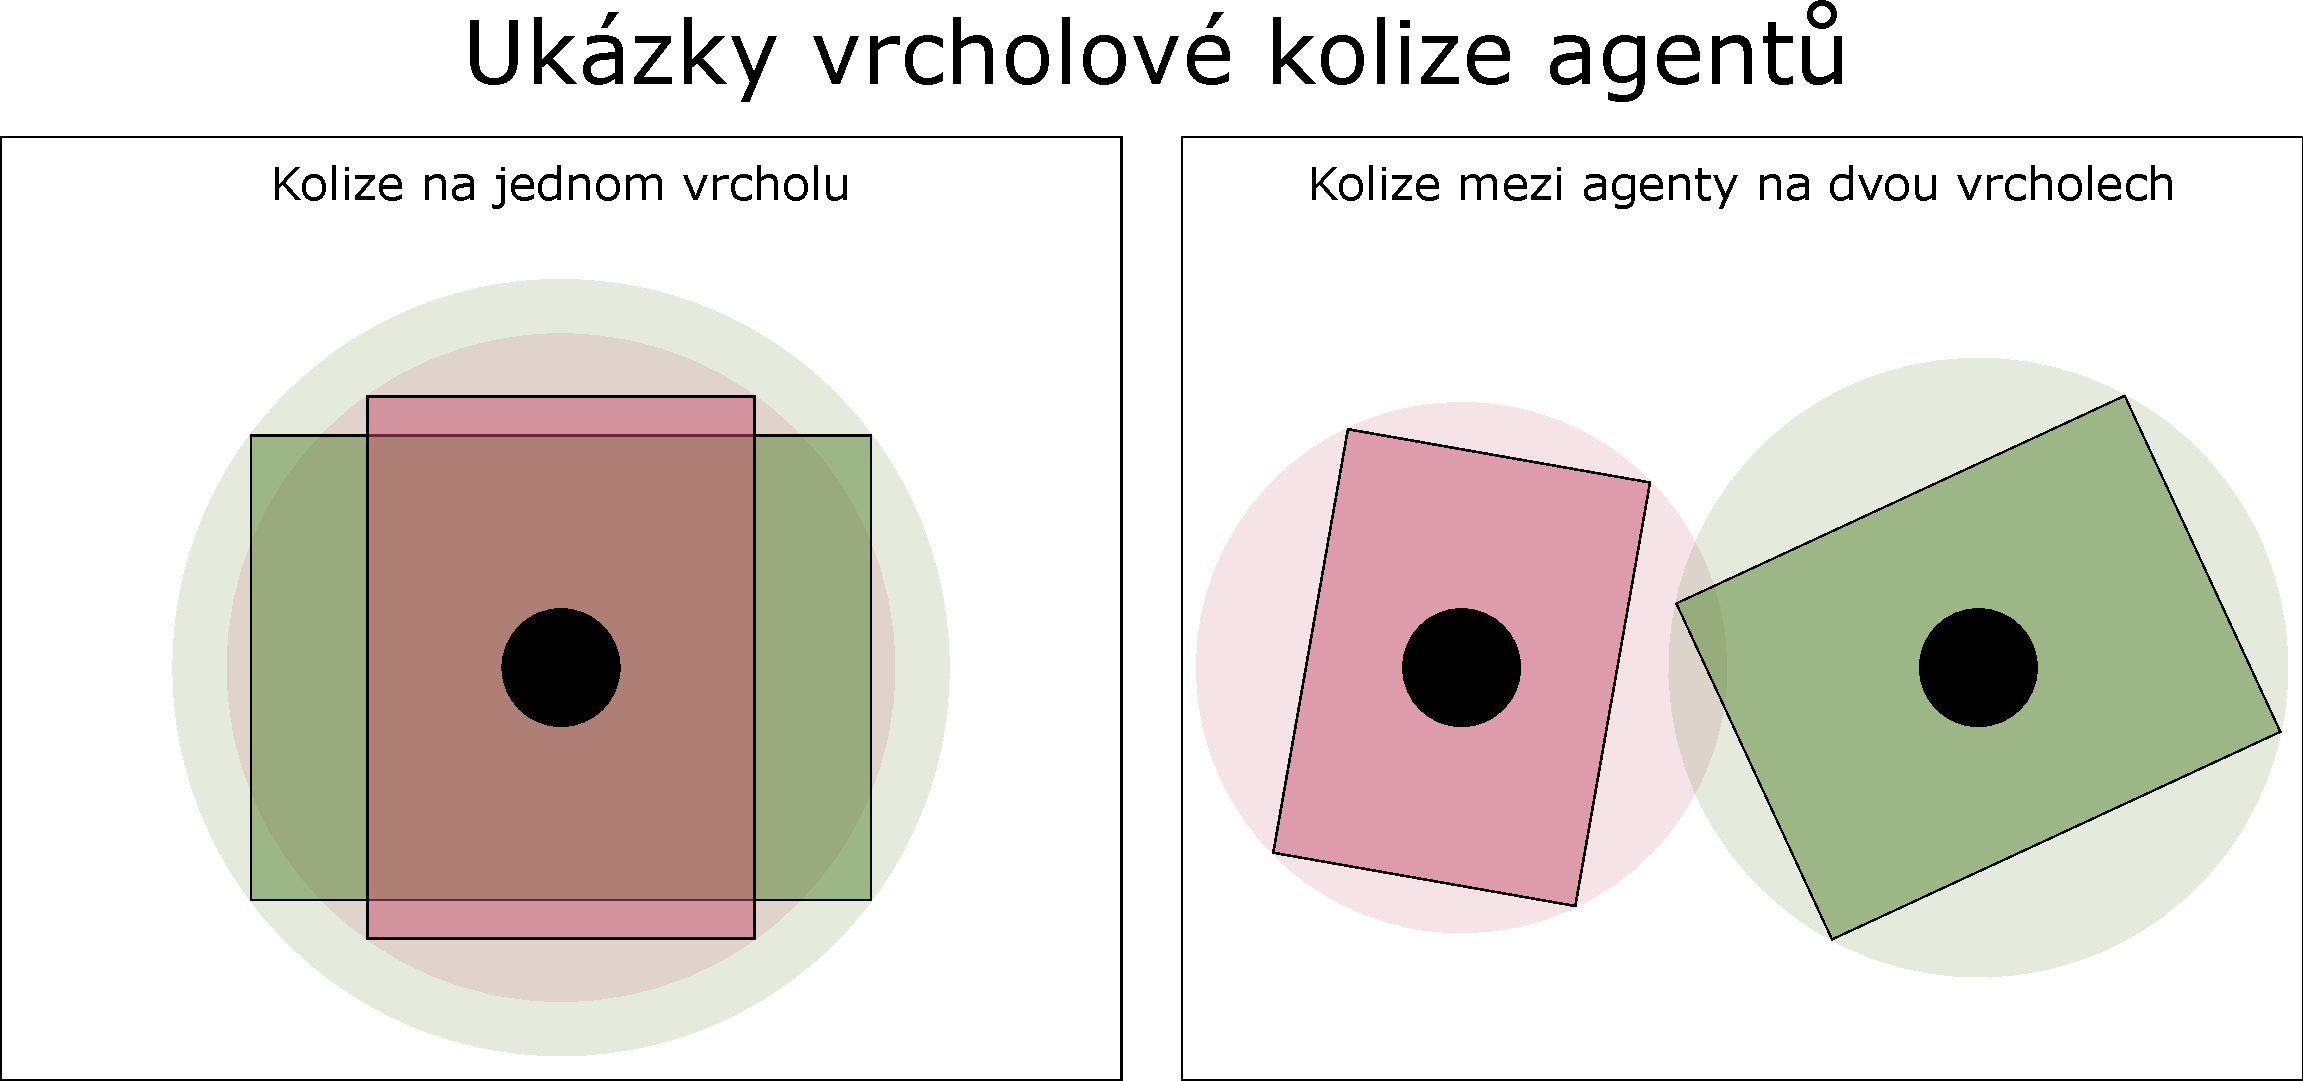
\includegraphics[width=\textwidth]{../img/kolize_vrchol}
  \caption{
    Ukázka kolizních situací, které jsou detekovány \hyperref[subsec:bezpecnost_vrcholu]{kontrolou bezpečnosti vrcholu}.
    Na obrázcích jsou černě zobrazeny vrcholy.
    Obdélníky reprezentují agenty a kruhy tvoří bezpečnou zónu příslušných agentů.
  }
  \label{fig:kolize_na_vrcholu}
\end{figure}

Níže je popsaný algoritmus na~kontrolu bezpečnosti vrcholu.
% @formatter:off
\begin{code}
// konstanty tabulka obsazených pozic t, minimální vzdálenost agentů d,
// maximální poloměr agenta m

// vstup krok s, vrchol v, poloměr agenta r
// výstup true pokud může agent být na v, jinak false
safe_vertex(s, v, r)
  for u in sorted(V, x -> dist(x, v))
    if dist(u, v) > r + m + d return true
    else
      n <- t[s][v]
      r' <- diameter(n)
      if dist(u, v) <= r + r' + d return false
  return true
\end{code}
% @formatter:on

\subsection{Cesta do~vrcholu}\label{subsec:cesta_do_vrcholu}

%Popis postupu kontroly, pseudokód, náčrtek.

\hyperref[subsec:cesta_do_vrcholu]{Kontrola cesty do vrcholu} zjišťuje,
zda~může plánovaný agent bezpečně přejet do~určeného vrcholu v~určitém kroku,
aniž by došlo ke kolizi s nějakým agentem opouštějícím daný vrchol.
Kontrola zahrnuje druhou \ref{str:mapf} podmínku
\uv{žádní dva agenti se nesmí projíždět stejnou hranou v jednom kroku} \eqref{eq:mapf_kolize_hrana}.
Avšak jelikož mají agenti nenulovou velikost, je nutné kontrolovat i případy, kdy agenti neprojíždí stejnou hranou.
Tyto situace jsou častější čím menší úhel je mezi sousedy vrcholu.
Například pro~čtvercový typ, kde je úhel mezi sousedy $90^\circ$, nastává tato kolize pouze pro velké agenty.
U~oktagonálního typu křižovatky dochází ke~kolizi mnohem častěji, protože úhel mezi sousedy činí $45^\circ$.
Ukázka kolizního stavu je zobrazena na obrázku (Obrázek~\ref{fig:kolize_cesta_do}).

\begin{figure}[h]
  \centering
  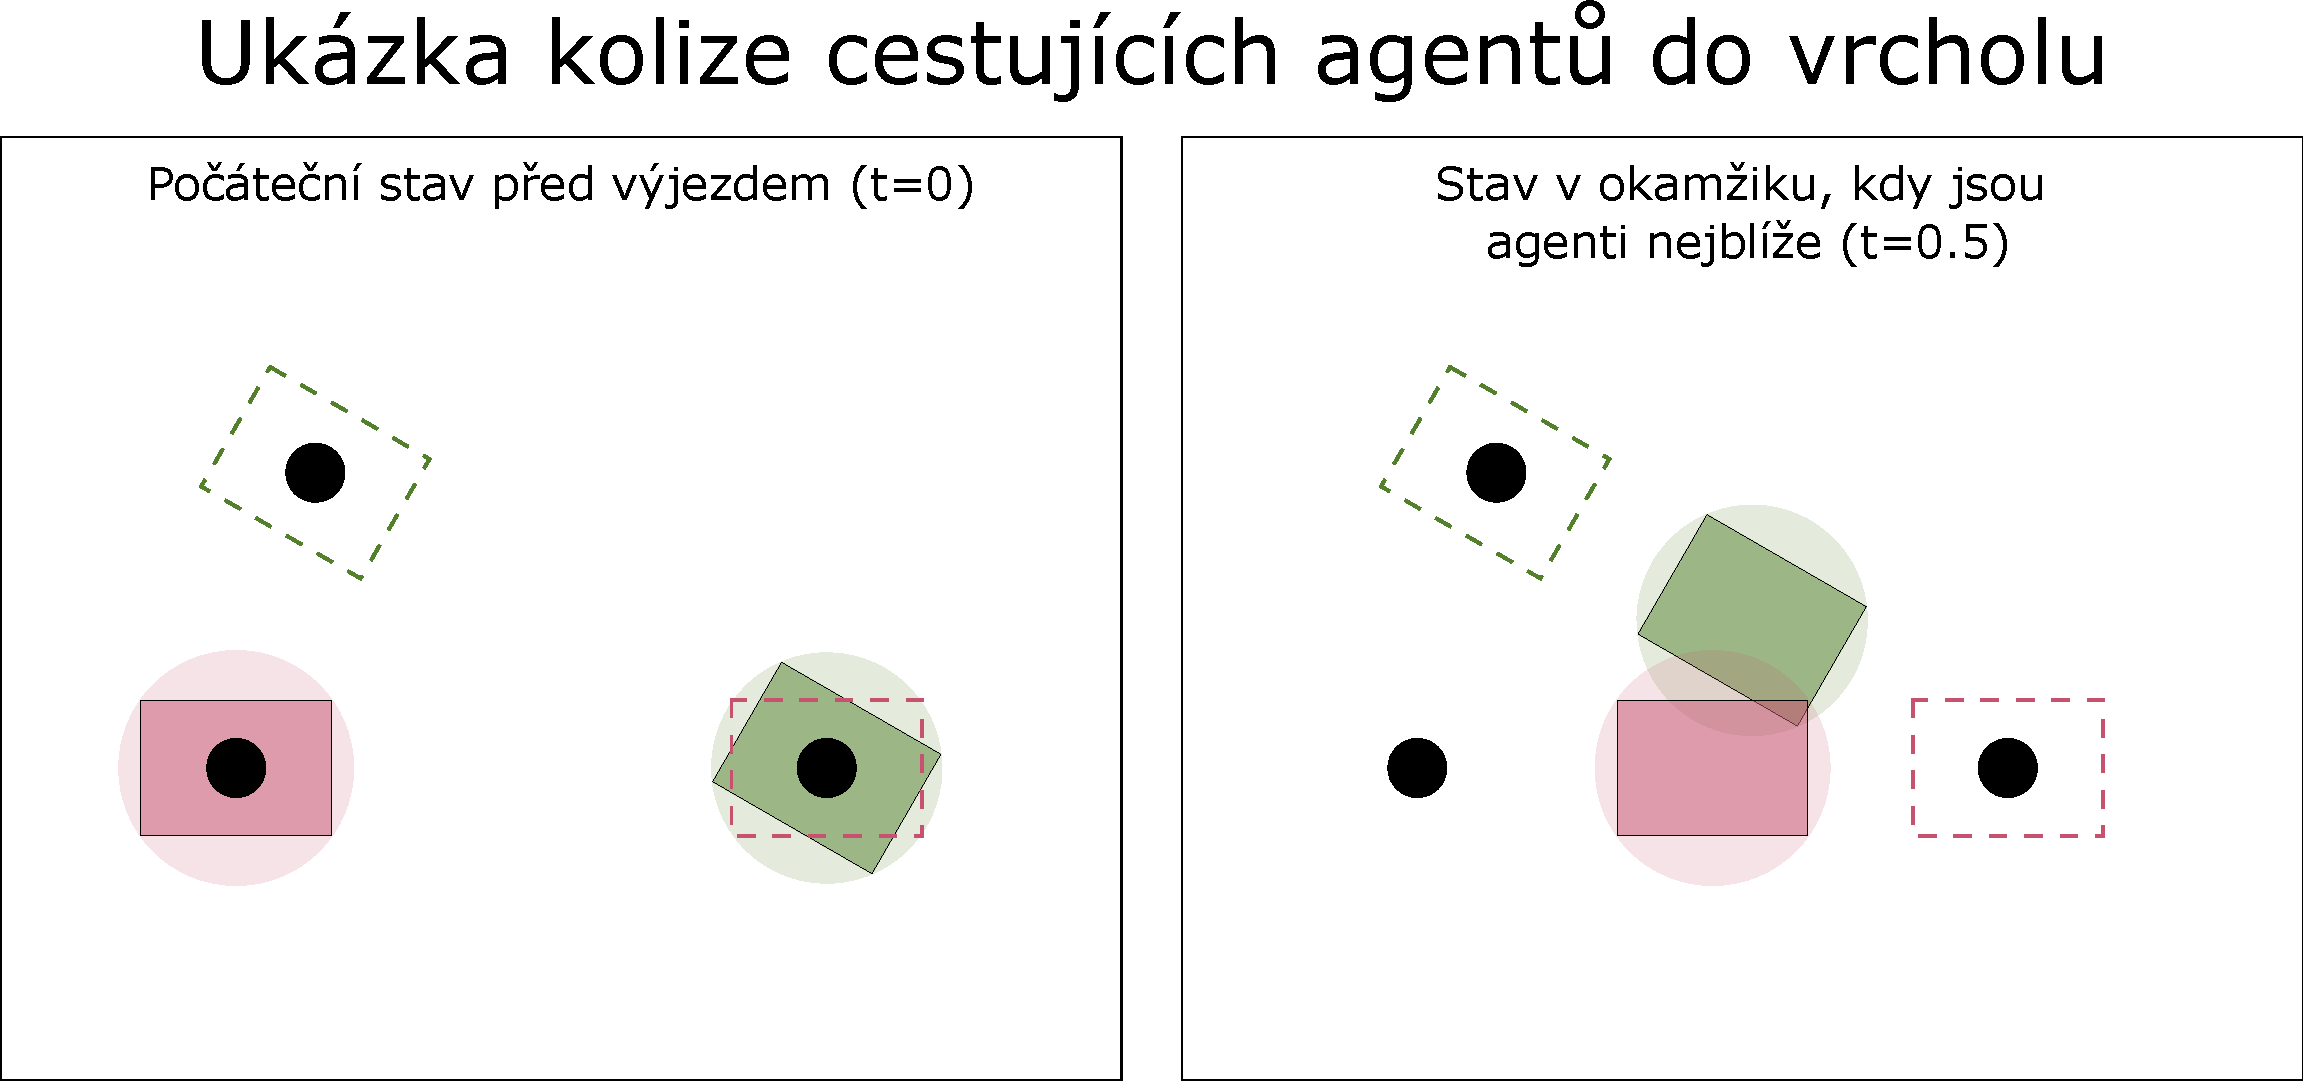
\includegraphics[width=\textwidth]{../img/kolize_cesta_do}
  \caption{
    Ukázka kolizní situace, která je detekována \hyperref[subsec:cesta_do_vrcholu]{kontrolou cesty do vrcholu}.
    Na obrázcích jsou černě zobrazeny vrcholy.
    Obdélníky reprezentují agenty a kruhy tvoří bezpečnou zónu příslušných agentů.
    Čárkované prázdné obdélníky značí cílové stavy agentů po jednom kroku.
  }
  \label{fig:kolize_cesta_do}
\end{figure}


Tato kontrola probíhá, pokud agent~$a$ opouští vrchol~$u$ v kroku~$s$ a přijíždí do~vrcholu~$v$ v následujícím kroku~$s + 1$.
Algoritmus nejprve zjistí, zda existuje naplánovaný agent~$b$, který je v~kroku~$s$ na~$v$.
Pokud žádný takový agent neexistuje, kontrola uspěje.
Jinak se zjistí vrchol~$w$, na~kterém se nachází agent~$b$ v~následujícím kroku $s + 1$.
Pokud nastane speciální případ $u=w$, odpovídá stav zmiňované \ref{str:mapf} podmínce \eqref{eq:mapf_kolize_hrana}.

Pokud se agenti srazí, musí být v kolizní poloze i v čase, kdy jsou sobě nejblíže.
Naopak pokud jsou dostatečně daleko i když jsou si nejblíže, při cestě nemůže dojít ke kolizi.
Jelikož kontrola zná pozice vrcholů $u$, $v$ a $w$, je schopna si dopočítat čas, ve~kterém se agenti nejvíce přiblíží.

Označím polohu agenta~$a$ jako $[x_a, y_a]$ a polohu agenta~$b$ jako $[x_b, y_b]$.
Stejným způsobem si označím pozice vrcholů $u$, $v$ a $w$ jako $[x_u, y_u]$, $[x_v, y_v]$ resp. $[x_w, y_w]$.
Dále si označím čas mezi kroky~$s$ a $s + 1$ jako~$t\in[0, 1]$.
Pro~$t = 0$ je poloha agenta~$a$ shodná s~pozicí vrcholu~$u$ a poloha agenta~$b$ shodná s~pozicí vrcholu~$v$.
Analogicky v~čase $t = 1$ se nachází agent~$a$ na~vrcholu~$v$ a agent~$b$ na~vrcholu~$w$.

Jelikož se agenti pohybují po~úsečce mezi vrcholy,
pro~$t\in[0, 1]$ se agent nachází na~$x_a = tx_u + (1 - t)x_v$, $y_a = ty_u + (1 - t)y_v$.
Poloha agenta~$b$ je analogicky $x_b = tx_v + (1 - t)x_w$ a $y_b = ty_v + (1 - t)y_w$.
Vzdálenost agentů v~závislosti na~čase~$t$ je $\sqrt{(x_a - x_b)^2 + (y_a - y_b)^2}$.
Dále upravím vzorec pod~odmocninou.
\begin{align*}
  ((x_a - x_b)^2 &+ (y_a - y_b)^2) = \\
  ((tx_u + (1 - t)x_v - tx_v - (1 - t)x_w)^2 &+ (ty_u + (1 - t)y_v - ty_v - (1 - t)y_w)^2) = \\
  ((tx_u + x_v - tx_v - tx_v - x_w + tx_w)^2 &+ (ty_u + y_v - ty_v - ty_v - y_w + ty_w)^2) = \\
  ((t(x_u - x_v - x_v + x_w) + x_v - x_w)^2 &+ (t(y_u - y_v - y_v + y_w) + y_v - y_w)^2) = \\
  (t(x_u - x_v - x_v + x_w) + x_v - x_w)^2 &+ (t(y_u - y_v - y_v + y_w) + y_v - y_w)^2 = \\
  (t(x_u - 2x_v + x_w) + x_v - x_w)^2 &+ (t(y_u - 2y_v + y_w) + y_v - y_w)^2 \\
\end{align*}

Pro~zjednodušení si označím
\begin{align*}
  x_0 &= x_u - 2x_v + x_w &\qquad
  x_1 &= x_w - x_v \\
  y_0 &= y_u - 2y_v + y_w &\qquad
  y_1 &= y_w - y_v
\end{align*}

Dosazením do~předchozího vzorce dostávám
\begin{align*}
  ((x_a - x_b)^2 &+ (y_a - y_b)^2) = \\
  (t(x_u - 2x_v + x_w) + x_v - x_w)^2 &+ (t(y_u - 2y_v + y_w) + y_v - y_w)^2 = \\
  (tx_0 - x_1)^2 &+ (ty_0 - y_1)^2
\end{align*}

Pro~nalezení nejmenší vzdálenosti zjistím čas~$t$, ve~kterém se agenti nacházejí nejblíže.
K~tomu spočítám derivaci vzdálenosti a zjistím, kdy je rovna nule.
Nejprve využiji faktu, že $\min\left(\sqrt{x}\right) = \min(x) \Rightarrow \frac{d}{dx} \sqrt {x} = 0 \leftrightarrow \frac{d}{dx} x=0$.
Následně
\begin{align}
  \frac{d}{dt} \sqrt{(x_a - x_b)^2 + (y_a - y_b)^2} &= 0 \nonumber \\
  \frac{d}{dt} ((x_a - x_b)^2 + (y_a - y_b)^2) &= 0 \nonumber \\
  \frac{d}{dt} ((tx_0 - x_1)^2 + (ty_0 - y_1)^2) &= 0 \nonumber \\
  \frac{d}{dt} (tx_0 - x_1)^2 + \frac{d}{dt} (ty_0 - y_1)^2 &= 0 \nonumber \\
  2(tx_0 - x_1)x_0 + 2(ty_0 - y_1)y_0 &= 0 \nonumber \\
  tx_0^2 - x_0 x_1 + ty_0 - y_0 y_1 &= 0 \nonumber \\
  t(x_0^2 + y_0^2) &= x_0 x_1 + y_0 + y_1 \label{eq:kol_d_dt}
\end{align}

Rozeberu dva případy podle podmínky
\begin{gather}
  x_0^2 + y_0^2 = 0\label{kol:nulova_podminka}
\end{gather}

Pokud je splněna podmínka~\ref{kol:nulova_podminka}, platí $x_0^2 = 0$ a $y_0^2 = 0$.
Odtud
\begin{align*}
  x_u - 2 x_v + x_w &= 0 \\
  x_u + x_w &= 2 x_v \\
  \frac{x_u + x_w}{2} &= x_v
\end{align*}
To je splněné jenom když $x_v$ je uprostřed $x_u$ a $x_w$.
Analogicky $y_0^2 = 0 \Leftrightarrow \frac{y_u + y_w}{2} = y_v$, tedy $y_v$ je uprostřed $y_u$ a $y_w$.
Obě tyto podmínky jsou splněny jenom když se vrchol~$v$ nachází přesně uprostřed úsečky z~$u$ do~$w$.

V~tom případě se agenti nepovoleně přiblíží pokud vzdálenost vrcholů $v$ a $w$ je menší než
součet poloměru agentů $d_a$ a $d_b$ a dovolené vzdálenosti mezi agenty \emph{safe distance}~$d$.
To~lze vyjádřit nerovností $(x_w - x_v)^2 + (y_w - y_v)^2 = x_1^2 + y_1^2 > (d_a + d_b + d)^2$.


Pokud podmínka~\ref{kol:nulova_podminka} neplatí, je možné spočítat čas~$t'$, kdy jsou agenti nejblíže vyjádřením z~\ref{eq:kol_d_dt}.
\begin{equation}
  \label{eq:kol_t}
  t' = \frac{x_0 x_1 + y_0 y_1}{x_0^2 + y_0^2}
\end{equation}

Po~dopočítání času spočítám vzdálenost agentů $a$ a $b$ v~čase~$t'$.
Rozdíl $x$-ové souřadnice agentů je roven
\begin{gather*}
  t' x_u + (1 - t')x_v - (t' x_v + (1 - t')x_w) =
  t' x_u + x_v - t' x_v - t' x_v - x_w + t' x_w = \\
  t'(x_u - 2x_v + x_w) + x_v - x_w =
  t' x_0 - x_1
\end{gather*}

Obdobně rozdíl $y$-ové souřadnice činí $t' y_0 - y_1$.
Pro~tento případ kontrola projde jenom pokud $(t' x_0 - x_1)^2 + (t' y_0 - y_1)^2 > (r_a + r_b + d)^2$.

Pro~výsledný algoritmus si nejdříve nadefinuji funkci $safe\_neighbour$.
Tato funkce pomocí postupu výše zkontroluje, zda-li dojde ke~kolizi mezi agenty $a$ a $b$
pokud už známe vrcholy $u$, $v$ a $w$.
% @formatter:off
\begin{code}
// konstanty bezpečná vzdálenost d

// agent a s poloměrem da cestuje z u do v,
// agent b s poloměrem db cestuje z v do w
safe_neighbour(v, u, w, da, db)
  if u is w return false

  x0 <- u.x - 2*v.x + w.x
  x1 <- w.x - v.x
  y0 <- y.u - 2*v.y + w.y
  y1 <- w.y - v.y

  // vzdálenost mezi středy agentů na druhou
  dist <- (da + db + d) ** 2

  if x0 is 0 and y0 is 0
    return x1 ** 2 + y1 ** 2 > dist

  else
    t' <- (x0 * x1 + y0 * y1 ) / (x0 ** 2 + y0 ** 2)
    x_diff <- (t' * x0 - x1) ** 2
    y_diff <- (t' * y0 - y1) ** 2
    return x_diff + y_diff > dist
\end{code}
\label{alg:check_neighbour}
% @formatter:on

Výsledný algoritmus kolize vypadá následovně.
% @formatter:off
\begin{code}
// konstanty tabulka obsazených pozic t

// agent a s poloměrem da cestuje z vrcholu u do v v kroku s
safe_step_to(s, u, v, da)
  b <- t[s][v]
  if b is Null return true

  w <- b.path[s + 1]
  db <- diameter(b)
  return safe_neighbour(v, u, w, da, db)
\end{code}
% @formatter:on


\subsection{Cesta z~vrcholu}\label{subsec:cesta_z_vrcholu}

Popis postupu kontroly, pseudokód.

%
%Poslední kontrola ověřuje opačný případ předchozí kontroly.
%Zjišťuje se, zda plánovaný agent~$a$ může bezpečně odjet z~vrcholu~$v$
%aniž by se srazil s~jiným agentem~$b$ cestujícím do~$v$.
%Kontrola probíhá podobně předchozímu případu, agent~$a$ cestuje z~$v$ do~$w$ v~kroku~$s$,
%agent~$b$ cestuje z~$u$ do~$v$ opět v kroku~$s$.
%
%Pro~kontrolu opět použiji funkci $safe\_neighbour$, akorát prohodím parametry.
%Výsledný algoritmus je následovný.
%% @formatter:off
%\begin{code}
%// konstanty tabulka obsazených pozic t
%
%// agent a s poloměrem da cestuje z vrcholu v do w v kroku s
%safe_step_from(s, v, w, da)
%  b <- t[s + 1][v]
%  if b is Null return true
%
%  u <- b.path[s]
%  db <- diameter(b)
%  return safe_neighbour(v, u, w, db, da)
%\end{code}
%% @formatter:on


\section{Safe lanes}\label{sec:safe_lanes}

%Převedení řešení \citet{Dresner} na graf.

%Parametry a pseudokód.

Algoritmus~\nameref{sec:safe_lanes} je založen na~křižovatkách s předem definovanými pruhy pro~auta.
Tímto způsobem řešení jsem se inspiroval u~práce \citet{Dresner}.
V~jejich práci používali jednu křižovatku s~danými pruhy.
Agentům dovolovali pouze měnit rychlost.
Já použiji jejich koncept jízdy v~pruzích, avšak moji agenti rychlost měnit nemůžou.

\citet{Dresner} plánování spadá pod \nameref{subsec:individualni_planovani}.
Plánují tedy agenty postupně jednoho po~druhém.
\nameref{sec:safe_lanes} algoritmus používá stejný přístup.
Prochází všechny přijíždějící agenty v~neurčitém pořadí a zkusí každému agentovi přiřadit nekolizní cestu.

Algoritmus~\nameref{sec:safe_lanes} se podívá na~pruh, popřípadě pruhy, podle vjezdu a výjezdu či~výjezdů daných agentem.
Pořadí procházení pruhů je dáno jeho délkou.
Délky jednotlivých pruhů si může algoritmus předem spočítat.
Pro~každý vrchol na~cestě dané pruhem provede algoritmus kontrolu popsanou v~předchozí kapitole~\ref{sec:kolize}.
Agentovi je přiřazena první nalezená nekolizní cesta.
Pokud taková cesta neexistuje, vjezd agenta je zamítnut.

Následující kód ukazuje plánování jednoho agenta.
% @formatter:off
\begin{code}
// konstanty tabulka obsazených pozic t, množina pruhů p

plan_agent(step, agent)
  r <- agent.diameter
  for exit in sorted(agent.exits, x -> dist(entry, x))
    path <- p[agent.entry, exit]
    last <- path[0]
    for i in 1, ..., path.length - 1
      s <- step + i - 1
      vertex = path[i]
      safe_transfer <- safe_transfer_set(s, last, vertex, r, t)
      if not safe_transfer
        continue
    agent.path <- path
    add_planned_agent(t, agent, s)  // přidám agenta do t
    return agent
  return NULL
\end{code}
% @formatter:on


\section{A*}\label{sec:a_star}

%Přesný popis A* algoritmu.

\nameref{sec:a_star} je známý prohledávací algoritmus pro~rychlé hledání nejkratších cest.
Algoritmus potřebuje znát prohledávací prostor určený možnými stavy.
Dále je nutné uvést určitou \emph{heuristiku}, která pro~určitý vrchol vrátí
spodní odhad na~cenu zbylé cesty z~aktuálního stavu do~cílového stavu.
Algoritmus si zároveň pamatuje pro~každý navštívený stav cenu cesty z~počátečního stavu do~aktuálního.
\nameref{sec:a_star} postupně prochází frontu navštívených stavů.
Při~procházení odebere stav z~fronty a poté pro~daný stav přidá sousední stavy do~fronty.
Vybraný stav z~fronty je určen nejmenším součtem cenou cesty
do~aktuálního stavu z~počátečního a heuristiky v~aktuálním stavu.
Tento součet je spodní odhad na~minimální cenu cesty z~počátku do~cíle vedoucí přes navštívené stavy,
přes~které byl aktuální vrchol dosažen.
\nameref{sec:a_star} zaručuje při~tomto postupu optimalitu nalezené cesty.

V~následujících kapitolách popíšu dvě různé implementace \nameref{sec:a_star} algoritmu pro~řešení problému křižovatky.

\subsection{Individuální A* (\ref{str:a_star_ars})}\label{subsec:individualni_a_star}\labeltext{A*RS}{str:a_star_ars}

%Popis úpravy A* algoritmu pro řešený problém, parametry a pseudokód.

\ref{str:a_star_ars} patří do~kategorie \ref{str:rs} algoritmů.
Plánuje stejně jako \nameref{sec:safe_lanes}, jednoho agenta po~druhém.
Akorát tentokrát algoritmus dovoluje agentům \uv{opustit} svoje~pruhy.

Pro~správné fungování \nameref{sec:a_star} je potřeba vhodně vybrat cenu cesty a heuristiku.
Cena cesty se počítá podobně jako při~hledání \hyperref[par:pruh]{pruhu} v~křižovatce.
Cena je složena z více kritérií, a to \hyperref[par:ars_vzdalenost]{vzdálenost},
\hyperref[par:ars_uhel_zataceni]{úhel zatáčení} a \hyperref[par:ars_pocet_zataceni]{počet zatáčení}.
Priorita kritérií je nejprve podle menší \hyperref[par:ars_vzdalenost]{vzdálenosti},
poté menšího \hyperref[par:ars_uhel_zataceni]{úhlu zatáčení}
a nakonec vyššího \hyperref[par:ars_pocet_zataceni]{počtu zatáček}.
Takto jsem se rozhodl, protože chci najít nejkratší cesty do~cíle.
Pokud existuje více stejně dlouhých cest do~cíle, chci vybrat nejvíce \uv{příjemnou} cestu pro~pasažéry auta.
Pokud má více cest všechny kritéria stejné, mají všechny stejnou cenu.

\paragraph{Vzdálenost}\label{par:ars_vzdalenost} je počet hran grafu, přes~které cesta vede.
Duplicitní hrany se započítávají vícekrát.
Pokud agent stojí na místě, vzdálenost se nemění.

\paragraph{Úhel zatáčení}\label{par:ars_uhel_zataceni} určuje úhel, o~který se musí agent při~sledování cesty otočit.
Pro~každý prostřední vrchol se na~cestě dopočítá úhel mezi hranami,
přes~kterou se agent na~vrchol dostal a kterou odjel.
Tento úhel se dá jednoduše geometricky dopočítat, jelikož známe přesnou pozici vrcholů.
\nameref{par:ars_uhel_zataceni} je součet absolutních hodnot těchto úhlů.

\paragraph{Počet zatáčení}\label{par:ars_pocet_zataceni} udává počet
nenulových \hyperref[par:ars_uhel_zataceni]{úhlů zatáčení}.

\paragraph{Heuristika}\label{par:ars_heuristika} v tomto případě je minimální počet hran cesty
z~aktuálního vrcholu do~nejbližšího z~cílových vrcholů.
Při~tomto výpočtu ignoruji všechny agenty na~křižovatce.
Pokud žádná taková cesta neexistuje, je hodnota \hyperref[par:ars_heuristika]{heuristiky} $\infty$.

Heuristika nebere v~úvahu úhel ani počet zatáčení.
Tato \hyperref[par:ars_heuristika]{heuristika} je přípustná, dokonce i~monotónní.

Prohledávací prostor jsou vrcholy křižovatky rozšířené o~krok, ve~kterém by agent na~daný vrchol přijel.
Následující stavy daného stavu jsou všechny validní stavy dané sousedy vrcholu aktuálního stavu.
Formálně pro~vrchol $u$ jsou jeho sousedi vrcholy $\{v \in V | (u,v)\in E\}$,
kde $V$ je množina vrcholů a $E$ je množina hran.

\subsubsection{Parametry}\label{subsubsec:ars_parametry}
Pro~reálnější pohyby agentů po~křižovatce je vhodné omezit množinu sousedů vrcholu.
Avšak určení vhodného omezení je komplikované.
Proto jsem se rozhodl umožnit omezení měnit parametry.
Zároveň parametry napomáhají rychlejšímu prohledávání omezením prohledávaného prostoru.
Bohužel při~nastavení parametrů algoritmus ztrácí svojí optimalitu.

\paragraph{Maximum návštěv vrcholu (\ref{par:ars_mnv})}\labeltext{MNV}{par:ars_mnv}
udává maximální počet výskytů libovolného vrcholu na~cestě.
Proto jsou validní hodnoty kladná celá čísla.
Nejreálnější hodnota parametru by byla $1$, není pro~auto moc přirozené jezdit ve~smyčkách.
Avšak vyšší hodnoty mohou vést k~obecně lepšímu řešení.
Na obrázku (Obrázek \ref{fig:ars_mnv_example}) je vyobrazen příklad takové situace.
Agent $a$ cestuje z $A$ do $B$, agent $b$ cestuje z $B$ do $C$.
Pokud by agenti mohli navštívit každý vrchol nejvýše jednou, neexistují nekolizní trasy pro~oba agenty najednou.
Avšak pokud povolíme alespoň dvě návštěvy vrcholu, existuje pro~agenta $a$ trasa $A, 1, 2, 1, 2, 3, 4, B$
a pro~agenta $b$ cesta $C, 4, 3, 2, 5, D$.

\begin{figure}[h]
	\centering
	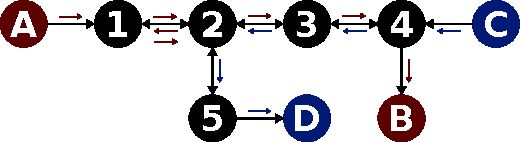
\includegraphics[width=140mm]{../img/mnv_example}
	\caption{Situace, při které neexistují cesty pro~oba agenty, aniž by se aspoň jeden vracel na navštívený vrchol}
	\label{fig:ars_mnv_example}
\end{figure}

\paragraph{Povolené zastavování (\ref{par:ars_pz})}\labeltext{PZ}{par:ars_pz}
určuje, zda-li může agent stát na~místě.
Formálněji pokud dovolím zastavování, vrchol se stane sám sobě sousedem a může se vyskytovat vícekrát na~cestě za~sebou.
Jednotlivé stání na~místě se pořád započítávají jako jednotlivé návštěvy,
tudíž maximální doma stání musí být menší než~hodnota \ref{par:ars_mnv}.

\paragraph{Maximální prodleva při~cestě (\ref{par:ars_mpc})}\labeltext{MPC}{par:ars_mpc}
omezuje počet kroků strávených agentem na~křižovatce.
Nalezená trasa pro daného agenta musí trvat nejvýše $\ref{par:ars_mpc} + p$ kroků,
kde $p$ je počet kroku optimální cesty (doba jízdy v~\hyperref[par:pruh]{pruhu}).
Hodnota $0$ znamená, že agent může jet pouze cestou stejného počtu kroků
jako je počet kroků jízdy v \hyperref[par:pruh]{pruhu}.
Tento parametr slouží jako omezení hloubky prohledávání.

\paragraph{Povolené vracení (\ref{par:ars_pv})}\labeltext{PV}{par:ars_pv}
může agentovi zakázat vracet~se na~vrchol, ze~kterého přijel.
Tento parametr dovoluje agentovi pouze \uv{jízdu dopředu}, což je přirozené od~jízdy v~autě očekávat.
Formálně pokud je tento parametr nenastaven, jsou zakázány cesty obsahující $u,v,v,\dots,v,u$,
kde $u, v \in V$ a $u \neq v$.
Posloupnost vrcholů $v$ musí být dlouhá alespoň jedna, avšak není zhora omezená.

\subsubsection{Sousední stavy}\label{subsubsec:sousedni_stavy}

Nyní blíže popíšu výběr následujícího stavu.
Přesněji popíšu funkci \ref{subsubsec:sousedni_stavy}\labeltext{\textrm{neighbour\_states}}{alg:sousedni_stavy},
která dostává na~vstup stav a vrací následující množinu platných stavů.
Množina následných stavů je ovlivněna \hyperref[subsubsec:ars_parametry]{parametry}.
Avšak většinou se jedná o~podmnožinu sousedních vrcholů aktuálního vrcholu, popřípadě ještě aktuální vrchol.
Tuto~množinu budu nazývat \emph{sousedi}\labeltext{sousedi}{str:ars_sousedi}.

Pro~získání \hyperref[str:ars_sousedi]{sousedů} začnu s~množinou všech vrcholů,
do~kterých vede hrana z~vrcholu aktuálního stavu.
Budu předpokládat, že tuto množinu je jednoduše možné získat z~grafu křižovatky.
Pokud je nastavený \hyperref[subsubsec:ars_parametry]{parametr} \ref{par:ars_pz},
přidám do~množiny \hyperref[str:ars_sousedi]{sousedů} aktuální vrchol.

Agent se nesmí srazit s~žádným jiným naplánovaným agentem při~jízdě do~sousedního vrcholu.
Kolizní přejezdy jsou detekovány způsobem popsaným v~sekci \nameref{sec:kolize}.

Pro~kontrolu \hyperref[subsubsec:ars_parametry]{parametru} \ref{par:ars_mnv}
je možné projít všechny předchozí stavy až po~počáteční
a odebrat všechny vrcholy vyskytující se alespoň \ref{par:ars_mnv} krát během tohoto průchodu.
Následující pseudokód zobrazuje přesnější postup odstraňování.

\labeltext{\textrm{control\_MNV}}{alg:ars_mnv}
% @formatter:off
\begin{code}[fontsize=\footnotesize]
// MNV předem nastavená hodnota maxima návštěv vrcholu

// vstup aktuální stav, množina sousedních vrcholů
// výstup množina sousedů navštívená nejvýše MNV - 1
control_MNV(state, neighbours)
  occurs <- empty // slovník návštěv vrcholů s implicitní hodnotou 0
  predecessor <- state
  while predecessor is not NULL
    occurs[predecessor.vertex] <- occurs[predecessor.vertex] + 1
    predecessor <- predecessor.parent
  for vertex in neighbours
    if occurs[vertex] >= MNV
      neighbours.remove(vertex)
  return neighbours
\end{code}
% @formatter:on

Pokud je hodnota \hyperref[subsubsec:ars_parametry]{parametru} \ref{par:ars_mpc} konečná,
je možné provést filtrování sousedních vrcholů podle nejkratší vzdálenosti ze~souseda do~nejbližšího cíle.
Tuto vzdálenost vím díky heuristice, která má stejnou hodnotu.
Nejprve si spočítám maximální krok cesty\labeltext{MKC}{str:ars_mkc} (\ref{str:ars_mkc}) pro~daného agenta.
Pokud sečtu aktuální plánovaný krok s~hodnotou heuristiky počátečního vrcholu, dostanu nejmenší krok,
ve~kterém se může agent dostat do~nejbližšího cíle.
\ref{str:ars_mkc} přiřadím součet této hodnoty a \ref{MPC}.
Jednoduše je vidět, že agent nemůže dorazit do~cíle po~kroku \ref{str:ars_mkc},
aniž~by porušil podmínku určenou parametrem \ref{alg:ars_mpc}.

Následně mohu zkontrolovat, jestli se agent může dostat ze~sousedního vrcholu
do~některého cíle do~kroku \ref{str:ars_mkc}.
Vzdálenost souseda do~nejbližšího cíle zjistím z~heuristiky.
Tudíž stačí porovnat součet kroku stavu a heuristiky souseda s~hodnotou \ref{str:ars_mkc}.
Přesný vzhled filtrace je popsán v následujícím pseudokódu.

\labeltext{\textrm{control\_MPC}}{alg:ars_mpc}
% @formatter:off
\begin{code}[fontsize=\footnotesize]
// MKC předem spočtená hodnota maximálního kroku cesty
// heuristics množina vzdáleností do nejbližšího cíle indexovaná vrcholy

// vstup aktuální stav, množina sousedních vrcholů
// výstup množina sousedů dostatečně blízkých cílům
control_MPC(state, neighbours):
  for vertex in neighbours
    if state.step + heuristics[vertex] >= MKC:
      neighbours.remove(vertex)
  return neighbours
\end{code}
% @formatter:on

Poslední filtrování sousedů probíhá pouze, pokud je nastaven
\hyperref[subsubsec:ars_parametry]{parametr} \ref{par:ars_pv}.
Opět lze při~kontrole využít procházení předchozích stavů.
Přesněji nejprve naleznu nejpozději navštívený vrchol před~aktuálním.
Pokud takový vrchol neexistuje, mohu skončit.
Jinak odeberu tento vrchol ze~sousedů.
Následující pseudokód zobrazuje přesnější průběh.

\labeltext{\textrm{control\_PV}}{alg:ars_pv}
% @formatter:off
\begin{code}[fontsize=\footnotesize]
// PV předem nastavená hodnota parametru povolení vrácení

// vstup aktuální stav, množina sousedních vrcholů
// výstup množina sousedů s odebraným předchozím vrcholem
control_PV(state, neighbours)
  if PV
    return neighbours
  predecessor <- state.parent
  while predecessor is not NULL and predecessor.vertex is state.vertex
    predecessor <- predecessor.parent
  if predecessor is not NULL
    neighbours.remove(predecessor.vertex)
  return neighbours
\end{code}
% @formatter:on

Nyní již můžu definovat funkci \ref{alg:sousedni_stavy} jako funkci, která vygeneruje validní sousední stavy.
Funkce nejprve pomocí funkce \textrm{neighbours} vygeneruje sousední vrcholy.
Poté~odstraní neplatné sousedy funkcemi \textrm{collision\_free},
\ref{alg:ars_mnv}, \ref{alg:ars_mpc} a \ref{alg:ars_pv}.
Nakonec pro~každý zbylý vrchol vytvoří nový stav.

Pro~vytvoření následujícího stavu je potřeba znát
úhel mezi vrcholy předchozího stavu, aktuálního stavu a dotyčného sousedního vrcholu.
Přesný výpočet zde vynechám.
Budu předpokládat, že se mohu zeptat grafu křižovatky na~tento úhel.

Pseudokód celkové funkce na~generování sousedních stavů je níže.


% @formatter:off
\begin{code}[fontsize=\footnotesize]
// G graf křižovatky
// funkce angle(u, v, w) na výpočet úhlu mezi třemi vrcholy
// heuristics množina vzdáleností do nejbližšího cíle indexovaná vrcholy

// vstup aktuální stav, poloměr agenta
// výstup množina sousedních stavů
neighbour_states(state, da)
  neighbours <- neighbours(state)
  neighbours <- collision_free(state, neighbours, da)
  neighbours <- control_MNV(state, neighbours)
  neighbours <- control_MPC(state, neighbours)
  neighbours <- control_PV(state, neighbours)

  current_vertex <- state.vertex
  last_vertex <- NULL
  if state.parent is not NULL
    last_vertex <- state.parent.vertex
  states <- empty

  for vertex in neighbours
    neighbour_state <- new
    neighbour_state.step <- state.step + 1
    if current_vertex is vertex
      neighbour_state.distance <- state.distance
    else
      neighbour_state.distance <- state.distance + 1

    angle <- 0
    if last_vertex is not NULL
      angle <- angle(last_vertex, current_vertex, vertex)
    neighbour_state.angle <- state.angle + angle
    if angle is 0
      neighbour_state.turns <- state.turns
    else
      neighbour_state.turns <- state.turns + 1
    neighbour_state.heuristics <- heuristics[vertex]
    states.add(neighbour_state)

  return states
\end{code}
% @formatter:on

\subsubsection{Výsledný algoritmus}\label{subsubsec:ars_vysledny_algoritmus}

Nakonec popíšu kompletní upravený \nameref{subsec:individualni_a_star} algoritmus.

Pro~zrychlení prohledávání použiji \emph{graph-search} variantu \nameref{sec:a_star} algoritmu.
V~této variantě si algoritmus pamatuje navštívené stavy (stavy odebrané z~fronty).
Z~množiny sousedních stavů je možné odebrat všechny navštívené stavy.
U tohoto algoritmu jsou stavy totožné, pokud mají stejný vrchol, stejný krok a zároveň vrcholy všech předků si odpovídají.
Nutnost shody všech předků vyplývá z použití dodatečných parametrů, které omezují množinu sousedů.
Například pokud se dostanu na stejný vrchol ve stejný krok ze dvou různých vrcholů
a povolím pouze jedno navštívení vrcholu, sousední stavy se u obou variant budou lišit.

Během testování jsem zjistil, že kontrola pouze rovnosti posledního vrcholu a předchozího stavu
značně zrychluje běh algoritmu, aniž by~se výrazně zhoršilo plánování.
Proto jsem se rozhodl udělat kompromis a určit, že dva stavy jsou si rovné právě tehdy,
když mají stejný vrchol, krok, a jejich rodiče mají stejný vrchol.

Nejprve je nutné pro~daného agenta spočítat heuristiku pro~každý vrchol.
To mohu provést procházením přes~cílové vrcholy.
Pro~každý cíl spočtu vzdálenost od~každého vrcholu do~tohoto cíle.
Pokud je tato hodnota menší než zatím nejmenší nalezená vzdálenost, přepíši tuto hodnotu.
Pro~účely počítání vzdálenosti mezi vrcholy si můžu tyto vzdálenosti uložit předem ke~grafu.
Tyto hodnoty lze získat například Floyd–Warshallovým algoritmem (\citet*{Floyd-Warshall}).
Poté se spočte hodnota posledního kroku \ref{str:ars_mkc} a uloží se pro~pozdější použití.

Následně algoritmus vygeneruje počáteční stav a přidá ho do~fronty prohledávaných stavů.
Poté~algoritmus odebere z~fronty nejmenší stav podle součtu ceny cesty do~vrcholu stavu a heuristiky.
Pokud vrchol odebraného stavu je mezi cílovými, zkonstruuje se cesta a přiřadí se agentovi.
Plánování agenta je v~tomto případě hotové, už~zbývá jen přidat naplánovanou cestu
do~\hyperref[par:obsazene_pozice]{tabulky obsazených pozic}, aby nedošlo ke~kolizi s~pozdějšími agenty.
Agent je následně vrácen zpět \hyperref[sec:simulace]{simulátoru}.

Pokud vrchol stavu není mezi cílovými,
získají se pomocí výše popsaného postupu sousední stavy a přidají se do~fronty.
Takto algoritmus pokračuje, dokud nenalezne validní cestu, nebo není fronta prázdná.
V~tom případě nemůže být agent naplánován, jeho cestování je pozdržené, a simulátoru se vrátí $NULL$.

Konstrukci cesty provedu postupným procházením předků koncového stavu.
Pro~každý takový stav přidám na~začátek cesty vrchol zmíněného stavu.
Tento postup budu opakovat, dokud nenarazím na předka s rodičem $NULL$.
Tento postup nazvu \ref{alg:ars_construct_path}\labeltext{\textrm{construct\_path}}{alg:ars_construct_path}.

% @formatter:off
\begin{code}[fontsize=\footnotesize]
// vstup finální stav cesty
// výstup kompletní cesta z vrcholů
construct_path(state)
  path <- empty
  while state is not NULL
    path.addFirst(state.vertex)
    state <- state.parent
\end{code}
% @formatter:on


Následující pseudokód zachycuje celý \nameref{subsec:individualni_a_star} algoritmus.

% @formatter:off
\begin{code}[fontsize=\footnotesize]
// G graf křižovatky se vzdálenostmi mezi vrcholy
// MPC parametr maximální prodlevy cesty

// vstup krok, plánovaný agent
// výstup agent nebo NULL
plan_agent(step, agent)
  MKC <- step + MPC + heuristics[entry]
  da <- agent.diameter

  // prioritní fronta porovnávající prvky podle součtu ceny cesty a heuristiky
  queue <- emptyPriorityQueue
  initial_state <- empty
  initial_state.vertex <- agent.entry
  initial_state.step <- agent.step
  initial_state.heuristics <- heuristics[entry]
  queue.push(initial_state)

  while not queue.empty()
    state <- queue.pop()
    if agent.exits.contain(state.vertex)
      agent.path <- construct_path(state)
      add_planned_agent(step, agent)  // přidání agenta do obsazených pozic
      return agent
    else
      queue.addAll(neighbour_states(state, da))

  return NULL
\end{code}
% @formatter:on


%\subsection{Hromadný A* (\ref{str:a_star_arsg})}\label{subsec:hromadny_a_star}\labeltext{A*RSG}{str:a_star_arsg}

%Rozšíření A* pro více agentů, popis vylepšení.
%Parametry, pseudokód.

Tento algoritmus plánuje agenty \ref{str:rsg} strategií, čili hledá cesty pro~všechny nové agenty najednou.
Algoritmus je založen na~\nameref{sec:a_star} algoritmu.

\subsubsection{Složený hromadný A*}\label{subsubsec:arsg_slozeny_hromadny}
Předchozí \ref{str:a_star_ars} algoritmus lze poměrně jednoduše rozšířit na~variantu pro~více agentů.
Pokud potřebuji naplánovat $n$ agentů, můžu rozšířit strukturu \ref{str:a_star_ars} stavu o~vrcholy,
na~kterých se nacházejí všichni agenti.
Tedy místo jednoho vrcholu by stav obsahoval $n$-tici vrcholů.
Stav je koncový, pokud všechny vrcholy jsou v~cílových vrcholech odpovídajících agentů.

Dále potřebuji upravit hodnotu \hyperref[par:ars_vzdalenost]{vzdálenosti} jako součet vzdáleností jednotlivých agentů.
Stejným způsobem upravím hodnoty \hyperref[par:ars_uhel_zataceni]{úhlu zatáčení},
\hyperref[par:ars_pocet_zataceni]{počtu zatáčení} a \hyperref[par:ars_heuristika]{heuristiky} jako součet
odpovídajících hodnot přes všechny agenty.

Při~vytváření následujících stavů určitého stavu je nutné zjistit \hyperref[str:ars_sousedi]{sousedy} vrcholů
jednotlivých agentů stejným způsobem jako u~\ref{str:a_star_ars} (sekce \ref{subsubsec:sousedni_stavy}).
Každý prvek kartézského součinu těchto množin \hyperref[str:ars_sousedi]{sousedů} tvoří vrcholy následujícího stavu.

Oproti \ref{str:a_star_ars} je navíc nutné kontrolovat kolize mezi jednotlivými plánovanými agenty.
Pokud je nalezená kolize mezi alespoň dvěma plánovanými agenty, je daný stav zamítnut.

Bohužel prohledávací prostor má velikost $|V|^n$, kde $n$ je počet plánovaných agentů.
Například pro~čtvercovou křižovatku s~\hyperref[par:velikost_krizovatky]{velikostí} $4$,
jedním \hyperref[par:vjezdy]{vjezdem} a jedním \hyperref[par:vyjezdy]{výjezdem} (Obrázek~\ref{fig:square_type_graph})
by~měl prohledávací prostor pro~jednoho agenta velikost $24$, pro~dva agenty $576$, pro~tři $13824$.
Proto je plánování pro~velký počet agentů je téměř nemožný z~časových i~paměťových důvodů.
Naštěstí byly vyvinuty techniky na~chytřejší plánování pomocí \nameref{sec:a_star}.



%\subsection{Vylepšený Hromadný A* (\ref{str:varsg})}\label{subsec:vylepseny_hromadny_a_star}\labeltext{VA*RSG}{str:varsg}

\citeauthor{Standley_2010} se zabýval zlepšením multiagentního \nameref{sec:a_star} algoritmu.
Nakonec ve~své práci \citet*{Standley_2010} sepsal techniky, které ve~většině případů výrazně zrychlily prohledávání.
Já se zaměřím pouze na~\nameref{subsubsec:varsg_independence_detection},
jelikož dle mého názoru přináší největší zrychlení.

\subsubsection{Independence Detection}\label{subsubsec:varsg_independence_detection}

Tato metoda rozdělí plánované agenty do~skupin.
Poté nalezne cesty pro~jednotlivé skupiny zvlášť bez~ohledu na~ostatní skupiny.
Když jsou všechny skupiny naplánovány, hledají se kolize mezi jednotlivými skupinami.
Pokud nejsou žádné kolize nalezeny, všichni agenti mají už naplánovanou validní cestu.
Jinak existuje kolize mezi agenty dvou skupin.

V~tom případě zkusí algoritmus přeplánovat první skupinu v~kolizi tak,
aby už žádný agent z~této skupiny neměl kolizní trasu s~žádným agentem první i druhé skupiny.
Pokud se nepodařilo takové trasy najít, algoritmus zkusí najít nové trasy pro~agenty druhé skupiny.
Jestliže se nepodařilo úspěšně přeplánovat ani druhou skupinu, spojí se obě skupiny do~jedné.
Potom se najdou trasy pro~tuto novou skupinu.
Při všech přeplánování se vždy kontrolují kolize s~agenty naplánovanými v~předešlých krocích.

Při~přeplánování by mohlo dojít k~zacyklení.
Například mám $3$ skupiny $g_1, g_2, g_3$, a $g_1$ je v kolizi s~$g_2$.
Povede se mi přeplánovat skupinu $g_1$,avšak nyní je $g_1$ v~kolizi s~$g_3$.
Po~opětovném přeplánování $g_1$ může oět dojít ke~kolizi s~$g_2$.
Proto je nutné udržovat si historii skupin, se kterými byla aktuálně plánovaná skupina v~kolizi.
Při~hledání nových tras se agenti vyhýbají nejen druhé skupině, ale i všem předešlým skupinám.

\paragraph{Illegal moves table}\label{par:varsg_illegal_moves_table} je datová struktura,
kterou algoritmus používá při~přeplánování k~hledání kolize s~agenty jiné skupiny.
Struktura této tabulky je shodná se strukturou \hyperref[par:obsazene_pozice]{tabulkou obsazených pozic}.
Tudíž mohu kontrolovat kolize přejezdu stejným způsobem popsaným v sekci \ref{sec:kolize}.

Před~každým přeplánováním skupiny si algoritmus uloží pro~každý krok množinu dvojic vrcholu a agenta.
Pro~každého agenta ze~skupiny z~historie nebo kolizní skupiny je do~tabulky přidána pro~každý krok, kdy agent cestuje,
dvojice zmíněného agenta a vrcholu z~jeho aktuální trasy, kde~se vyskytuje ve~zmíněný krok.

Kontrola sousedních vrcholů pro~jednoho agenta probíhá podobně jako při~kontrole u~\ref{str:a_star_ars}.
Avšak kromě kontroly kolize s~naplánovanými agenty pomocí \hyperref[par:obsazene_pozice]{tabulkou obsazených pozic}
se totožnými kontrolami zaručuje nekolizní přejezd s~agenty jiných skupin pomocí
\hyperref[par:varsg_illegal_moves_table]{Illegal moves table}.

K~rychlejšímu naplánování chceme minimalizovat počet přeplánování.
Proto by bylo vhodné již při~plánování skupiny preferovat cesty,
které mají co~nejméně kolizních tras s~ostatními skupinami.
Přesněji je důležitý počet agentů jiných skupin, které kolidují s~některým agentem aktuální skupiny.
Avšak pro~zaručení optimality je nutné dodržovat stejné uspořádání jako při~\nameref{str:a_star_arsg}.
Porovnání na~počet kolizních agentů tedy budu používat jenom tehdy, mají-li stavy totožnou
\hyperref[par:ars_vzdalenost]{vzdálenost}, \hyperref[par:ars_uhel_zataceni]{úhlu zatáčení},
\hyperref[par:ars_pocet_zataceni]{počtu zatáčení} i \hyperref[par:ars_heuristika]{heuristiku}.
Pokud bude shodný i~počet agentů s~kolizní trajektorií, budu upřednostňovat stavy s~menším počtem celkových kolizí.
Při~tomto součtu už započítávám stejného agenta vícekrát.

\paragraph{Conflict avoidance table}\label{par:varsg_conflict_avoidance_table} je tabulka, pomocí níž
algoritmus zjišťuje množství těchto kolizí.
Strukturou je podobná struktuře \nameref{par:varsg_illegal_moves_table}.
Agenti jiných skupin mohou ale být v~kolizi, proto může být naplánováno více agentů na~stejném vrcholu ve~stejný krok.
Proto je výhodnější pamatovat si místo dvojice vrchol-agent dvojici vrchol-množina agentů.
Zjišťování kolizních agentů lze opět provést podobnými způsoby popsanými v sekci \nameref{sec:kolize}.
Rozdíl je jenom namísto kontrolování s~jedním agentem
se musí zkontrolovat kolize se všemi agenty v~dané množině.

Algoritmus potřebuje na~začátku výpočtu rozdělit agenty do~skupin.
Vhodný způsob rozdělení je přiřazení každému agentovi svojí skupinu,
protože složitost plánování roste exponenciálně s~množstvím agentů ve~skupině.
Všichni agenti jsou naplánováni zvlášť stejným stejně jako u~\ref{str:a_star_ars}.
Pokud nějaký agent nemůže být naplánován, je jeho skupina vyřazena.

Může se stát, že algoritmus nebude moci najít trasy pro~všechny agenty po~spojení dvou skupin.
V~tom případě je nutné vyřadit určité agenty ze~skupiny.
Pro~zachování co nejlepších výsledků jsem se rozhodl, že budu zkoušet všechny podmnožiny agentů dané skupiny,
dokud algoritmus nenalezne trasy pro~danou podmnožinu.

\subsubsection{Parametry}\label{subsubsec:arsg_parametry}
Algoritmus má opět několik nastavitelných parametrů, kterými je možné ovlivnit chování a složitost výpočtu.
Jelikož je algoritmus rozšířením \nameref{str:a_star_ars}, ponechávám algoritmu všechny tyto parametry.
Omezení parametrem platí pro~všechny plánované agenty ve~skupině.

Počet podmnožin agentů u~spojování skupin je exponenciální.
Při~testování jsem zjistil, že algoritmu občas zabere hodně času najít vhodnou podmnožinu.
Proto jsem se rozhodl dovolit algoritmu použít zjednodušený výpočet.
Zjednodušený výpočet znamená, že algoritmus místo spojování skupin ponechá pouze skupinu větší velikosti.

\paragraph{Zjednodušený výpočet po (\ref{par:arsg_zvp})}\labeltext{ZVP}{par:arsg_zvp} je jediný nový parametr.
Tento parametr udává, po jak dlouhé prodlevě (ms) má algoritmus začít používat zjednodušené počítání.

\subsubsection{A*OID}\label{subsubsec:a_star_aoid}
Další způsob řešení \nameref{subsubsec:online_mapf} problému je pomocí \ref{str:oid} algoritmu.
Při~tomto způsobu řešení se v~novém kroku plánují nejen noví agenti, ale i agenti již naplánovaní.
Tento způsob by měl dávat lepší výsledky než \ref{str:varsg}.
Ale přirozeně vzroste počet plánovaných agentů, což vede ke~zpomalení výpočtu.
Proto \ref{str:oid} používá strategii \uv{neměnit plány agentů, pokud není potřeba}.
Znamená to, že naplánovaní agenti se znovu neplánují, jestliže nekolidují s~novými agenty.

\nameref{str:varsg} algoritmus lze jednoduše rozšířit na~\ref{str:oid} variantu.
Na~začátku každému naplánovanému agentovi přidělíme vlastní skupinu.
Avšak oproti novým agentům pro ně prvotní cestu nehledáme, jelikož už jsou naplánovaní předchozími kroky.
Akorát jejich aktuální cesta nezačíná ve~vrcholu vjezdu,
ale obecným vrcholem podle toho, kde se v~plánovaný krok nacházejí.
Množina koncových vrcholů je stejná.

Poté může algoritmus pokračovat stejně jako v~\ref{str:a_star_arsg}.
Jediný rozdíl je u~slučování dvou skupin.
Algoritmus si nemůže dovolit odebrat agenta z~výpočtu a zamítnout ho, jelikož už je částečně naplánován.
Z~tohoto důvodu se při~slučování skupin neprochází všechny podmnožiny agentů skupin,
ale jenom podmnožiny obsahující všechny dříve naplánované agenty.

Algoritmus opět podporuje \hyperref[par:arsg_zvp]{zjednudušený výpočet}.
Avšak tentokrát namísto ponechávání větší skupiny
algoritmus skupiny spojí do~jedné a odebere všechny nově plánované agenty.
Zbylí agenti již byli naplánovaní v~předešlých krocích, tudíž jim algoritmus přiřadí zpět poslední platné cesty.
Tyto cesty jsou vzájemně nekolizní, jelikož jsou výsledkem předešlých úspěšných plánování.

Abych snížil počet přeplánovaných agentů, rozhodl jsem se přidat algoritmu dva nastavitelné parametry.

\paragraph{Maximální počet agentů (\ref{par:aoid_mpa})}\labeltext{MPA}{par:aoid_mpa} určuje,
s~kolika agenty může algoritmus nanejvýš počítat.
Algoritmus přidá k~novým agentům tolik naplánovaných, abych jejich součet nepřekročil tuto hodnotu.
Výběr agentů pro~plánování tedy probíhá ještě před započtením výpočtu tras.
Agenti se berou od~nejnovějšího po~nejstarší.

\paragraph{Počet přeplánovaných kroků (\ref{par:aoid_ppk})}\labeltext{PPK}{par:aoid_ppk}
omezuje stáří přeplánovaných agentů.
Z~vybraných agentů na~přeplánování jsou odebráni takoví, kteří už cestují déle než hodnota tohoto parametru.


%\subsection{Conflict-Based Search (\ref{str:cbs})}\label{subsec:conflict_based_search}\labeltext{CBS}{str:cbs}

%Popis algoritmu, úprava pro můj problém.
%Parametry, pseudokód.

\nameref{subsec:conflict_based_search} algoritmus \citep*{Sharon} rozšiřuje jakýkoliv \ref{str:rs} algoritmus
na multiagentní plánování.
V mém případě budu rozšiřovat \ref{str:a_star_ars}.

\ref{str:cbs} začíná individuálním naplánováním všech agentů nezávisle na~sobě.
Čili agenti nesmějí mít kolize s~již cestujícími agenty,
avšak mohou mí kolizní trajektorii s~jinými aktuálně plánovanými agenty.
Poté se zkontroluje, zda-li nemají nějací agenti kolizní trajektorie.
Pokud ne, plánování úspěšně končí.
Jinak se prohledávání rozdělí na dva případy.
V obou případech je přeplánován jeden agent s podmínkou, že se musí vyhnout koliznímu místu.
Poté se opakuje opětovné hledání kolizí a rozdělování na případy.
Aby nedošlo k zacyklení, je nutné při plánování agenta vyhnout se nejen aktuální kolizi, ale také všem předchozím.
Výpočet postupně vytváří strom,
kde každý vrchol obsahuje cesty agentů (mohou být navzájem kolizní) a tabulku zakázaných pozic.
Algoritmus skončí v~prvním nalezeném vrcholu neobsahujícím kolizní trasy.

Již cestující agenti mohou omezovat trasy natolik, že pro agenta neexistuje žádná nekolizní cesta skrze křižovatku.
Dále se může stát, že agent nenajde žádnou nekolizní cestu, která by nevedla místo, které bylo dříve označené jako kolizní.
V obou případech plánování tohoto agenta selže a agent zcela odstraněn z~vrcholu.
Následně jsou nalezeni agenti, kteří byli v~historii přeplánováni kvůli odstraněnému agentovi.
Pro~tyto agenty jsou nalezeny nové cesty, jelikož pro~ně může existovat lepší cesta.

Algoritmus postupně prochází listy stromu výpočtu.
Pořadí průchodu je určeno počtem agentů.
Pokud je počet agentů u~více listů shodný, vybere se vrchol s nejmenší vzdáleností podobně jako u \ref{str:a_star_arsg}.
Algoritmus naplánuje pouze agenty, kteří mají cesty ve~vybraném listu, vjezd zbylých agentů je zamítnut.

\ref{str:cbs} najde optimální cestu pro všechny agenty \citep{Sharon}.
Avšak velikost stromu může být obrovská.
Proto jsem se rozhodl obětovat optimalitu a zjednodušit práci algoritmu, pokud plánování trvá příliš dlouhou dobu.
Ve zjednodušeném režimu algoritmus přeplánuje takovým způsobem, aby neměl žádné kolize s ostatními plánovanými agenty.
To znamená, že v tomto režimu plánuje algoritmus agenty stejně jako \ref{str:a_star_ars}.


\subsubsection{Parametry}\label{subsubsec:cbs_parametry}

\nameref{subsubsec:cbs_parametry} algoritmu jsou stejné jako u \ref{str:varsg} a mají podobný význam.
Hodnoty Maximum návštěv vrcholu (\ref{str:ars_mnv}), Povolené zastavování (\ref{str:ars_pz}),
Maximální prodleva při~cestě (\ref{str:ars_mpc}) a Povolené vracení (\ref{str:ars_pv})
algoritmus používá při~plánování jednoho agenta.
Tyto \hyperref[subsubsec:ars_parametry]{parametry} ovlivňují plánování stejně jako u \ref{str:a_star_ars}.
Hodnota parametru \ref{str:arsg_zvp} opět určuje po jak dlouhé prodlevě má algoritmus přejít na zjednodušené plánování.

\subsection{CBS-OID}\label{subsec:cbsoid}

\ref{str:cbs} lze podobně jako \ref{str:varsg} rozšířit na \ref{str:suboid} variantu.
K plánovaným agentů se přidají agenti z předchozích kroků.
Jako počáteční cesty těchto agentů se použijí jejich již naplánované trasy, tudíž se znova nepočítají.
Výpočet je poté shodný, až na~případy, kdy pro~ně nebyla nalezena cesta.
Pokud k~takové situaci dojde, namísto odstranění agenta se odstraní celý list ze~stromu výpočtu.

Parametry jsou rozšířené stejně jako u \nameref{subsubsec:a_star_aoid} o~Maximální počet agentů (\ref{str:aoid_mpa})
a Počet přeplánovaných kroků (\ref{str:aoid_ppk}).
Význam těchto parametrů je shodný.



\section{SAT planner}\label{sec:sat_planner}

%Definice SAT a MAXSAT, popis řešiče.
%Rozdíl mezi optimálním ohodnocením a splňujícím ohodnocením.
%
%Popis převodu problému na SAT.
%Popis parametrů a odhad na počet proměnných a počet klauzulí.
%
%Pseudokód.

SAT je známý a prozkoumaný problém, na který existují vysoce optimalizované řešiče.
Proto není úplně zcestné pokusit se problém křižovatky převést na SAT problém.

SAT\labeltext{SAT}{str:sat} se zabývá problémem určení,
zda-li existuje splňující ohodnocení výrokových proměnných logické formule.
Vstupní hodnotou je tedy výroková formule a výstupem ohodnocení proměnných takové,
že daná formule je splněná, popřípadě oznámení o nesplnitelnosti formule.
Zadaná formule většinou bývá v konjunktivní normální formě (\ref{str:sat_cnf})\labeltext{CNF}{str:sat_cnf}, což je konjunkce klauzulí.
Klauzule jsou disjunkce literálů a literál je výroková proměnná, nebo její negace.
Například formule v \ref{str:sat_cnf} pro proměnné $p_1, \dots, p_{10}$ může být
\[
	\bigwedge_{i=1}^{7}(p_i \vee p_{i+1} \vee p_{i + 3}).
\]

MAXSAT je rozšíření \ref{str:sat}.
Klauzule jsou rozdělené na dvě skupiny,
\ref{str:sat_hard}\labeltext{\emph{hard}}{str:sat_hard} a \ref{str:sat_soft}\labeltext{\emph{soft}}{str:sat_soft}.
Aby bylo ohodnocení splňující, musí být splněny všechny \ref{str:sat_hard} klauzule.
Úkolem řešiče je nalézt splňující ohodnocení, které maximalizuje počet splněných \ref{str:sat_soft} klauzulí.
Tento problém je očividně těžší, jelikož nestačí najít libovolné řešení, ale to nejlepší.

Vážený MAXSAT přidává navíc možnost přiřadit \ref{str:sat_soft} klauzulím váhy.
Řešič se nesnaží maximalizovat počet splněných klauzulí, ale součet jejich vah.

Pokud chceme naplánovat agenty pomocí váženého MAXSAT, stačí převést plánování do \ref{str:sat_cnf}.
Převedení \ref{str:mapf} problému na \ref{str:sat_cnf} bylo mnohokrát popsáno \citep{bartak}.
Z tohoto postupu budu vycházet.

\subsection{Převod do \ref{str:sat_cnf}}\label{subsec:sat_prevod_do_cnf}

Vhodný začátek převodu je nadefinování výrokových proměnných.
Poté popíšu tvorbu klauzulí.

\subsubsection{Výrokové proměnné}\label{subsubsec:sat_vyrokove_promenne}

Vytvořím si výrokové proměnné pro každého agenta, pro každý krok a pro každý vrchol grafu.
Pokud se agent $a$ vyskytuje v čase $t$ na vrcholu $v$, je výroková proměnná $p_{t,a,v}$ pravdivá, jinak je nepravdivá.
Avšak abych nedostal nekonečnou \ref{str:sat_cnf}, určím si maximální dobu cesty \ref{par:sat_mpk}.
Čas v~proměnné je počet kroků od~plánovaného kroku a má hodnotu ${0, \dots, mpk}$
Počet výrokových proměnných je celkem $(mpk + 1) * |A| * |V|$, kde $A$ je množina agentů a $V$ množina vrcholů.

\subsubsection{\ref{str:sat_hard} Podmínky}\label{subsubsec:sat_hard_podminky}

V této kapitole popíšu způsob, jak vytvořit odpovídající \ref{str:sat_cnf}.
Avšak nebudu popisovat jednotlivé klauzule.
Namísto toho popíšu tvorbu klauzulí jednoduššími výrazy (např.\ pro každé $p_i$, maximálně jeden z $p_i$, \ldots).
Převod těchto výrazů do validní \ref{str:sat_cnf} je triviální.
Pokud formule obsahuje některou funkci, je možné funkci vyhodnotit předem a daný výraz přidat, pokud to má smysl.

Agent přijede na vrchol \hyperref[par:vjezdy]{vjezdu} v kroku příjezdu, pokud bude úspěšně naplánován.
Zároveň musí být v jednom z časů ~cíli, aby byla cesta kompletní.
Z toho vyplývá první podmínka pro každého agenta, která značí, že daný agent není v počáteční čas na vjezdu,
nebo je v jenom jeden čas na právě jednom výjezdu.
Matematicky:
\[
	(\forall_{a \in A}) \left(\neg p_{0,a,a_e} + \sum_{t=1}^{mpk} \sum_{f \in a_f} p_{t, a, f} = 1\right),
\]
kde $a_e$ je vrchol vjezdu agenta $a$ a $a_f$ jeho výjezdy.

Agent se nemůže nacházet na více vrcholech najednou.
Jinými slovy může být pro jednoho agenta a jeden čas maximálně jedna proměnná pravdivá:
\[
	(\forall a \in A)(\forall t \in {0, \dots, mpk})\left(\sum_{v=1}^{|V|} p_{t,a,v} \leq 1\right).
\]

Pokud je agent v určitý krok na vrcholu $v$, musí být v dalším kroku na některým vrcholu z jeho sousedů $N(v)$.
Množina sousedů může obsahovat i samotný vrchol $v$,
pokud \hyperref[par:sat_povolene_zastavovani]{povolíme zastavování}.
Toto platí až na vrcholy výjezdu, které opět pro agenta $a$ označím $a_f$, a také to neplatí pro poslední krok.
Matematickým zápisem tomu odpovídá podmínka
\[
	(\forall a \in A)(\forall t \in {0, \dots, mpk - 1})
	(\forall v \in V \setminus a_f)(p_{t,a,v} \rightarrow \vee_{n \in N(v)} (p_{t+1,a,n})).
\]

Počítání lze zrychlit zakázáním neplatných kombinací času a vrcholu.
Pro tyto účely si označím $d(u, v)$ jako délku nejkratší cesty mezi vrcholy $u$ a $v$.
Pokud mezi nimi cesta neexistuje, je hodnota $\infty$.
Agent nemůže být v čase $t$ na vrcholu vzdáleném více než $t$, jelikož se tam nemá jak dostat.
Stejně tak nemůže být v čase $t$ na vrcholu, který má vzdálenost k nejbližšímu cíli větší než $mpk - t$,
protože potom neexistuje způsob, jak se dostat do cíle včas.
Odtud plynou podmínka
\begin{gather*}
(\forall a \in A)(\forall t \in {0, \dots, mpk})(\forall v \in V)
	\\
	((d(a_e, v) > t \vee (\min_{f \in a_f} d(v, f) > mpk - t)) \rightarrow \neg p_{t, a, v}).
\end{gather*}

Nadále je nutné vyhnout se cestujícím agentům.
K tomu opět využiji funkci na kontrolu kolizí.
Projdu všechny vrcholy a pro každého agenta zjistím,
na kterých vrcholech se nesmí nacházet pomocí funkce \ref{alg:kol_prejezd_mnozina}:
\[
	(\forall a \in A)(\forall t \in {0, \dots, mpk - 1})(\forall u \in V)(\forall v \in N(u))
	(\neg \ref{alg:kol_prejezd_mnozina}(a_p + t, u, v, a_d, T) \rightarrow \neg p_{t, a, u}),
\]
kde $a_p$ je krok příjezdu agenta a $a_d$ je jeho \hyperref[par:polomer_agenta]{poloměr}
a $T$ je \nameref{par:obsazene_pozice}.

Poslední nutná podmínka je zamezení kolizím mezi plánovanými agenty.
Je nutné projít všechny dvojice agentů a poté všechny kombinace vrcholů a jejich sousedů.
Pokud se vrcholy nacházejí moc blízko, nemůžou se agenti vyskytovat na patřičných vrcholech v jeden čas.
Pro zjištění vzdáleností mohu využít tabulky \ref{str:kol_vzdalenosti} a \ref{str:kol_serazene_vzdalenosti}.
Tabulka \ref{str:kol_vzdalenosti} má uložené pro každé možné dva přejezdy nejbližší vzdálenosti mezi trasami
(\ref{subsec:kontrola_prejezdu_jeden_agent}).
Tabulka \ref{str:kol_serazene_vzdalenosti} má uložené pro každé dva sousední vrcholy $u$ a $v$
seřazené dvojice vrchol, vzdálenosti podle nejmenší vzdálenosti (\ref{subsec:kontrola_prejezdu_mnozina_agentu}).
Pseudokód zachycující tvorbu této podmínky:

% @formatter:off
\begin{code}[fontsize=\footnotesize]
// tabulka seřazených vzdáleností sort_dist
// minimální povolená vzdálenost agentů d
// množina vrcholů V

// seznam agentů A
add_agents_clauses(A)
  for i in 1, ..., |A|
    for j in 1, ..., i - 1
      a <- A[i]
      b <- A[j]
      d_safe = a.polomer + b.polomer + d
      for u in V
        for v in N(u)
          for p, p_dist in sort_dist[u][v]
            if p_dist > d_safe
              break
            for q in N(p)
              if d_safe <= distance[u][v][p][q]
                for t in 0, ..., mpk - 1
                  add_hard_clause(not_near(t, a, u, v, b, p, q))
\end{code}
% @formatter:on

V kódu výše používám funkci $add\_hard\_clause(not\_near(t, a, u, v, b, p, q))$,
která přidá do SAT řešiče hard podmínku $(p_{t,b,p} \wedge \_{t+1,b,q}) \rightarrow (\neg p_{t,a,u \vee p_{t+1,a,v}})$.
Tato podmínka znamená, že pokud cestuje agent $b$ v čase $t$ z $p$ do $q$,
potom nesmí agent $a$ cestovat ve stejný čas z $u$ do $v$.

\subsubsection{\ref{str:sat_soft} Podmínky}\label{subsubsec:sat_soft_podminky}

Podobně jako u všech předešlých algoritmech budu optimalizovat \ref{str:soc} metriku.
U každému agenta tedy budu chtít co nejdřívější příjezd do cíle.
Proto vytvořím jednoprvkové klauzule pro každého agenta a pro každý vrchol s cenou určenou časem.
Klauzuli v čase $t$ ($p_{t, a, v}$) přidělím váhu $mpk - t + 1$.
Tím bude mít příjezd v $t = 1$ váhu $mpk$ a v čase $t = mpk$ váhu $1$.

Abych maximalizoval počet naplánovaných agentů, vytvořím ještě pro každého agenta $a$
klauzuli $p_{0, a, a_e}$ s vahou alespoň $(mpk + 2) * (|A| - 1)$, kde $a_e$ je vrchol vjezdu agenta $a$.

\subsection{Parametry}\label{subsec:sat_parametry}

Aby byl algoritmus porovnatelný s ostatními algoritmy, přidal jsem podobné parametry použité v předešlých algoritmech.

\paragraph{Maximální počet kroků (\ref{par:sat_mpk})}\labeltext{MPK}{par:sat_mpk}
udává maximální délku plánu pro všechny agenty.

\paragraph{Maximum návštěv vrcholu (\ref{par:ars_mnv})} má stejný význam jako
parametr \ref{par:ars_mnv} u \hyperref[subsubsec:ars_parametry]{parametrů \ref{str:a_star_ars}}.
Hodnota udává maximální počet výskytů jednoho vrcholu na cestě.
Vzorcem $(\forall a \in A)(\forall v \in V)(\sum_{t=0}^{mpk} p_{t, a, v} \leq 1)$.

\paragraph{Povolené zastavování (\ref{par:ars_pz})}\label{par:sat_povolene_zastavovani} je taktéž vzatý
z \hyperref[subsubsec:ars_parametry]{parametrů \ref{str:a_star_ars}}.
Pokud je tento parametr nastaven, agent může stát na~místě.
Znamená to přidání vrcholu do množiny sousedů daného vrcholu.

\paragraph{Maximalizace} určuje, zda-li má řešič hledat libovolné splňující ohodnocení,
nebo maximalizovat váhu klauzulí.
Vypnutí optimalizace značně zrychluje výpočet, avšak může vést k mnohem horším výsledkům.
Jelikož jsem dovolil zamítnout agentovi vjezd, je možné všechny \ref{str:sat_hard} podmínky splnit
nastavením všech proměnných na $false$.

\subsection{SAT-RSG}\label{subsec:sat_rsg}
Jak název napovídá, algoritmus plánuje všechny nové agenty v daném kroku.
Počet proměnných činí na $|A| * |V| * (mpk + 1)$.
Jelikož počet proměnných vzroste lineárně, počet všech možných ohodnocení vzroste exponenciálně.
Po nalezení splňujícího ohodnocení se algoritmus podívá na proměnnou $p_{0, a, a_e}$ pro každého plánovaného agenta $a$.
Pokud je $false$, vjezd agenta je zamítnut.
Jinak se projdou všechny ostatní proměnné, a vyberou se pravdivé.
Z těch se podle $t$ sestaví cesta do prvního cíle.
Mohlo by se stát, že některé proměnné jsou nastaveny na $true$ i po čase příjezdu do cíle.
Tyto proměnné algoritmus ignoruje.


\subsection{SAT-RA}\label{subsec:sat_ra}

Plánování může proběhnout i pro již naplánované agenty pro nalezení lepších tras strategií \ref{str:ra}.
Avšak je nutné změnit určité podmínky.
Symbol $a_e$ u dříve naplánovaných agentů nese význam vrcholu, na kterém se v plánovaném kroku nachází agent.
Zároveň agent již vjel na křižovatku.
Proto je nutné zaručit, že bude naplánován.
To lze provést odstraněním $\neg p_{0, a, a_e}$ z první \ref{str:sat_hard} podmínky.
Dostanu tedy zjednodušenou podmínku:
\[
	(\forall_{a \in A}) \left(\sum_{t=1}^{mpk} \sum_{f \in a_f} p_{t, a, f} = 1\right).
\]

Zbytek algoritmu je stejný s \nameref{subsec:sat_rsg}.


%	%%% Fiktivní kapitola s ukázkami sazby

\chapter{Nápověda k~sazbě}


\section{Úprava práce}

Vlastní text bakalářské práce je uspořádaný hierarchicky do kapitol a podkapitol, každá kapitola začíná na nové straně.
Text je zarovnán do bloku.
Nový odstavec se obvykle odděluje malou vertikální mezerou a odsazením prvního řádku.
Grafická úprava má být v~celém textu jednotná.

Práce se tiskne na bílý papír formátu A4. Okraje musí ponechat dost místa na vazbu:
doporučen je horní, dolní a pravý okraj $25\,\textrm{mm} $, levý okraj $40\,\rm mm$.
Číslují se všechny strany kromě obálky a informačních stran na začátku práce;
první číslovaná strana bývá obvykle ta s~obsahem.

Písmo se doporučuje dvanáctibodové ($12\,\rm pt$) se standardní vzdáleností mezi řádky
(pokud píšete ve Wordu nebo podobném programu, odpovídá tomu řádkování $1,5$; v~\TeX{}u
není potřeba nic přepínat). Pro běžný text používejte vzpřímené patkové písmo.
Text matematických vět se obvykle tiskne pro zdůraznění skloněným (slanted) písmem,
není-li k~dispozici, může být zastoupeno kurzívou.

Primárně je doporučován jednostranný tisk (příliš tenkou práci lze obtížně svázat).
Delší práce je lepší tisknout oboustranně a přizpůsobit tomu velikosti okrajů:
$40\,\rm mm$ má vždy \emph{vnitřní} okraj. Rub titulního listu zůstává nepotištěný.

Zkratky použité v textu musí být vysvětleny vždy u prvního výskytu zkratky (v~závorce nebo
v poznámce pod čarou, jde-li o složitější vysvětlení pojmu či zkratky). Pokud je zkratek
více, připojuje se seznam použitých zkratek, včetně jejich vysvětlení a/nebo odkazů
na definici.

Delší převzatý text jiného autora je nutné vymezit uvozovkami nebo jinak vyznačit a řádně
citovat.


\section{Jednoduché příklady}

Čísla v~českém textu obvykle sázíme v~matematickém režimu s~desetinnou čárkou:
%%% Bez \usepackage{icomma}:
% $\pi \doteq 3{,}141\,592\,653\,589$.
%%% S \usepackage{icomma}:
$\pi \doteq 3,141\,592\,653\,589$.
V~matematických textech se považuje za přípustné používat desetinnou tečku
(pro lepší odlišení od čárky v~roli oddělovače). Numerické výsledky se uvádějí
s~přiměřeným počtem desetinných míst.

Mezi číslo a jednotku patří úzká mezera: šířka stránky A4 činí $210\,\rm mm$, což si
pamatuje pouze $5\,\%$ autorů. Pokud ale údaj slouží jako přívlastek, mezeru vynecháváme:
$25\rm mm$ okraj, $95\%$ interval spolehlivosti.

Rozlišujeme různé druhy pomlček:
červeno-černý (krátká pomlčka),
strana 16--22 (střední),
$45-44$ (matematické minus),
a~toto je --- jak se asi dalo čekat --- vložená věta ohraničená dlouhými pomlčkami.

V~českém textu se používají \uv{české} uvozovky, nikoliv ``anglické''.

% V tomto odstavci se vlnka zviditelňuje
	{
	\def~{{\tt\char126}}
	Na některých místech je potřeba zabránit lámání řádku (v~\TeX{}u značíme vlnovkou):
	u~předložek (neslabičnych, nebo obecně jednopísmenných), vrchol~$v$, před $k$~kroky,
	a~proto, \dots{} obecně kdekoliv, kde by při rozlomení čtenář \uv{ško\-brt\-nul}.
}


\section{Matematické vzorce a výrazy}

Proměnné sázíme kurzívou (to \TeX{} v~matematickém módu dělá sám, ale
nezapomínejte na to v~okolním textu a také si matematický mód zapněte).
Názvy funkcí sázíme vzpřímeně. Tedy například:
$\var(X) = \E X^2 - \bigl(\E X \bigr)^2$.

Zlomky uvnitř odstavce (třeba $\frac{5}{7}$ nebo $\frac{x+y}{2}$) mohou
být příliš stísněné, takže je lepší sázet jednoduché zlomky s~lomítkem:
$5/7$, $(x+y)/2$.

Nechť
\[   % LaTeXová náhrada klasického TeXového $$
	\mathbb{X} = \begin{pmatrix}
								 \T{\bm x_1} \\
								 \vdots      \\
								 \T{\bm x_n}
	\end{pmatrix}.
\]
Povšimněme si tečky za~maticí. Byť je matematický text vysázen
ve~specifickém prostředí, stále je gramaticky součástí věty a~tudíž je
zapotřebí neopomenout patřičná interpunkční znaménka. Výrazy, na které
chceme později odkazovat, je vhodné očíslovat:
\begin{equation}
	\label{eq01:Xmat}
	\mathbb{X} = \begin{pmatrix}
								 \T{\bm x_1} \\
								 \vdots      \\
								 \T{\bm x_n}
	\end{pmatrix}.
\end{equation}
Výraz \eqref{eq01:Xmat} definuje matici $\mathbb{X}$. Pro lepší čitelnost
a~přehlednost textu je vhodné číslovat pouze ty výrazy, na které se
autor někde v~další části textu odkazuje. To jest, nečíslujte
automaticky všechny výrazy vysázené některým z~matematických
prostředí.

Zarovnání vzorců do několika sloupečků:
\begin{alignat*}{3}
	S(t) &= \pr(T > t),    &\qquad t&>0       &\qquad&\text{ (zprava spojitá),}\\
	F(t) &= \pr(T \leq t), &\qquad t&>0       &\qquad&\text{ (zprava spojitá).}
\end{alignat*}

Dva vzorce se spojovníkem:
\begin{equation}
	\label{eq01:FS}
	\left.
	\begin{aligned}
		S(t) &= \pr(T > t) \\[1ex]
		F(t) &= \pr(T \leq t)
	\end{aligned}
	\;  % zde pomůže ručně vynechat trochu místa
	\right\}
	\quad t>0 \qquad \text{(zprava spojité).}
\end{equation}

Dva centrované nečíslované vzorce:
\begin{gather*}
	\bm Y = \mathbb{X}\bm\beta + \bm\varepsilon, \\[1ex]
	\mathbb{X} = \begin{pmatrix}
								 1 & \T{\bm x_1} \\ \vdots & \vdots \\ 1 &
								 \T{\bm x_n}
	\end{pmatrix}.
\end{gather*}
Dva centrované číslované vzorce:
\begin{gather}
	\bm Y = \mathbb{X}\bm\beta + \bm\varepsilon, \label{eq02:Y}\\[1ex]
	\mathbb{X} = \begin{pmatrix}
								 1 & \T{\bm x_1} \label{eq03:X} \\ \vdots & \vdots \\ 1 &
								 \T{\bm x_n}
	\end{pmatrix}.
\end{gather}

Definice rozdělená na dva případy:
\[
	P_{r-j}=
	\begin{cases}
		0, & \text{je-li $r-j$ liché},\\
		r!\,(-1)^{(r-j)/2}, & \text{je-li $r-j$ sudé}.
	\end{cases}
\]
Všimněte si použití interpunkce v této konstrukci. Čárky a tečky se
dávají na místa, kam podle jazykových pravidel patří.

\begin{align}
	x& = y_1-y_2+y_3-y_5+y_8-\dots = && \text{z \eqref{eq02:Y}} \nonumber\\
	& = y'\circ y^* = && \text{podle \eqref{eq03:X}} \nonumber\\
	& = y(0) y' && \text {z Axiomu 1.}
\end{align}


Dva zarovnané vzorce nečíslované:
\begin{align*}
	L(\bm\theta) &= \prod_{i=1}^n f_i(y_i;\,\bm\theta), \\
	\ell(\bm\theta) &= \log\bigl\{L(\bm\theta)\bigr\} =
	\sum_{i=1}^n \log\bigl\{f_i(y_i;\,\bm\theta)\bigr\}.
\end{align*}
Dva zarovnané vzorce, první číslovaný:
\begin{align}
	L(\bm\theta) &= \prod_{i=1}^n f_i(y_i;\,\bm\theta), \label{eq01:L} \\
	\ell(\bm\theta) &= \log\bigl\{L(\bm\theta)\bigr\} =
	\sum_{i=1}^n \log\bigl\{f_i(y_i;\,\bm\theta)\bigr\}. \nonumber
\end{align}

Vzorec na dva řádky, první řádek zarovnaný vlevo, druhý vpravo, nečíslovaný:
\begin{multline*}
	\ell(\mu,\,\sigma^2) = \log\bigl\{L(\mu,\,\sigma^2)\bigr\} =
	\sum_{i=1}^n \log\bigl\{f_i(y_i;\,\mu,\,\sigma^2)\bigr\}= \\
	= -\,\frac{n}{2}\,\log(2\pi\sigma^2) \,-\,
	\frac{1}{2\sigma^2}\sum_{i=1}^n\,(y_i - \mu)^2.
\end{multline*}

Vzorec na dva řádky, zarovnaný na $=$, číslovaný uprostřed:
\begin{equation}
	\label{eq01:ell}
	\begin{split}
		\ell(\mu,\,\sigma^2) &= \log\bigl\{L(\mu,\,\sigma^2)\bigr\} =
		\sum_{i=1}^n \log\bigl\{f(y_i;\,\mu,\,\sigma^2)\bigr\}= \\
		& = -\,\frac{n}{2}\,\log(2\pi\sigma^2) \,-\,
		\frac{1}{2\sigma^2}\sum_{i=1}^n\,(y_i - \mu)^2.
	\end{split}
\end{equation}


\section{Definice, věty, důkazy, \dots}

Konstrukce typu definice, věta, důkaz, příklad, \dots je vhodné
odlišit od okolního textu a~případně též číslovat s~možností použití
křížových odkazů. Pro každý typ těchto konstrukcí je vhodné mít
v~souboru s~makry (\texttt{makra.tex}) nadefinované jedno prostředí,
které zajistí jak vizuální odlišení od okolního textu, tak
automatické číslování s~možností křížově odkazovat.

\begin{definice}
	\label{def01:1}
	Nechť náhodné veličiny $X_1,\dots,X_n$ jsou definovány na témž
	prav\-dě\-po\-dob\-nost\-ním prostoru $(\Omega,\,\mathcal{A},\,\pr)$. Pak
	vektor $\bm X = \T{(X_1,\dots,X_n)}$ nazveme \emph{náhodným
	vektorem}.
\end{definice}

\begin{definice}[náhodný vektor]
	\label{def01:2}
	Nechť náhodné veličiny $X_1,\dots,X_n$ jsou definovány na témž
	pravděpodobnostním prostoru $(\Omega,\,\mathcal{A},\,\pr)$. Pak
	vektor $\bm X = \T{(X_1,\dots,X_n)}$ nazveme \emph{náhodným
	vektorem}.
\end{definice}
Definice~\ref{def01:1} ukazuje použití prostředí pro sazbu definice
bez titulku, definice~\ref{def01:2} ukazuje použití prostředí pro
sazbu definice s~titulkem.

\begin{veta}
	\label{veta01:1}
	Náhodný vektor $\bm X$ je měřitelné zobrazení prostoru
	$(\Omega,\,\mathcal{A},\,\pr)$ do $(\R_n,\,\mathcal{B}_n)$.
\end{veta}

\begin{lemma}
	[\citealp{Andel07}, str. 29]
	\label{veta01:2}
	Náhodný vektor $\bm X$ je měřitelné zobrazení prostoru
	$(\Omega,\,\mathcal{A},\,\pr)$ do $(\R_n,\,\mathcal{B}_n)$.
\end{lemma}
\begin{dukaz}
	Jednotlivé kroky důkazu jsou podrobně popsány v~práci \citet[str.
	29]{Andel07}.
\end{dukaz}
Věta~\ref{veta01:1} ukazuje použití prostředí pro sazbu matematické
věty bez titulku, lemma~\ref{veta01:2} ukazuje použití prostředí pro
sazbu matematické věty s~titulkem. Lemmata byla zavedena v~hlavním
souboru tak, že sdílejí číslování s~větami.

%	%%% Fiktivní kapitola s ukázkami citací

\chapter{Odkazy na literaturu}

Odkazy na literaturu vytváříme nejlépe pomocí příkazů
\verb|\citet|, \verb|\citep| atp.
(viz {\LaTeX}ový balíček \textsf{natbib}) a~následného použití
Bib{\TeX}u. V~matematickém textu obvykle odkazujeme stylem \uv{Jméno
autora/autorů (rok vydání)}, resp. \uv{Jméno autora/autorů [číslo
odkazu]}. V~českém/slovenském textu je potřeba se navíc vypořádat
s~nutností skloňovat jméno autora, respektive přechylovat jméno
autorky. Je potřeba mít na paměti, že standardní příkazy
\verb|\citet|, \verb|\citep|
produkují referenci se jménem autora/autorů v~prvním pádě a~jména
autorek jsou nepřechýlena.

Pokud nepoužíváme bib\TeX{}, řídíme se normou ISO 690 a zvyklostmi
oboru.

Jména časopisů lze uvádět zkráceně, ale pouze v~kodifikované podobě.


\section{Několik ukázek}

Mezi nejvíce citované statistické články patří práce Kaplana a~Meiera a~Coxe
\citep{KaplanMeier58, Cox72}. \citet{Student08} napsal článek o~t-testu.

Prof. Anděl je autorem učebnice matematické statistiky
\citep[viz][]{Andel98}. Teorii odhadu se věnuje práce
\citet{LehmannCasella98}. V~případě odkazů na specifickou informaci
(definice, důkaz, \dots) uvedenou v~knize bývá užitečné uvést
specificky číslo kapitoly, číslo věty atp. obsahující požadovanou
informaci, např. viz \citet[Věta 4.22]{Andel07} nebo \citep[viz][Věta
4.22]{Andel07}.

Mnoho článků je výsledkem spolupráce celé řady osob. Při odkazování
v~textu na článek se třemi autory obvykle při prvním výskytu uvedeme
plný seznam: \citet*{DempsterLairdRubin77} představili koncept EM
algoritmu. Respektive: Koncept EM algoritmu byl představen v~práci
Dempstera, Lairdové a~Rubina \citep*{DempsterLairdRubin77}. Při každém
dalším výskytu již používáme zkrácenou verzi:
\citet{DempsterLairdRubin77} nabízejí též několik příkladů použití EM
algoritmu. Respektive: Několik příkladů použití EM algoritmu lze
nalézt též v~práci Dempstera a~kol. \citep{DempsterLairdRubin77}.

U~článku s~více než třemi autory odkazujeme vždy zkrácenou formou:
První výsledky projektu ACCEPT jsou uvedeny v~práci Genbergové a~kol.
\citep{Genberget08}. V~textu \emph{nenapíšeme}: První výsledky
projektu ACCEPT jsou uvedeny v~práci \citet*{Genberget08}.

%	%%% Fiktivní kapitola s ukázkami tabulek, obrázků a kódu

\chapter{Tabulky, obrázky, programy}

Používání tabulek a grafů v~odborném textu má některá společná
pravidla a~některá specifická. Tabulky a grafy neuvádíme přímo do
textu, ale umístíme je buď na samostatné stránky nebo na vyhrazené
místo v~horní nebo dolní části běžných stránek. \LaTeX\ se o~umístění
plovoucích grafů a tabulek postará automaticky.

Každý graf a tabulku
očíslujeme a umístíme pod ně legendu. Legenda má popisovat obsah grafu
či tabulky tak podrobně, aby jim čtenář rozuměl bez důkladného
studování textu práce.

Na každou tabulku a graf musí být v~textu odkaz
pomocí jejich čísla. Na příslušném místě textu pak shrneme ty
nejdůležitější závěry, které lze z~tabulky či grafu učinit. Text by
měl být čitelný a srozumitelný i~bez prohlížení tabulek a grafů a
tabulky a grafy by měly být srozumitelné i~bez podrobné četby textu.

Na tabulky a grafy odkazujeme pokud možno nepřímo v~průběhu běžného
toku textu; místo \emph{\uv{Tabulka~\ref{tab03:Nejaka} ukazuje, že
muži jsou v~průměru o~$9,9\,\rm kg$ těžší než ženy}} raději napíšeme
\emph{\uv{Muži jsou o~$9,9\,\rm kg$ těžší než ženy (viz
Tabulka~\ref{tab03:Nejaka})}}.


\section{Tabulky}

\begin{table}[b!]

	\centering
%%% Tabulka používá následující balíčky:
%%%   - booktabs (\toprule, \midrule, \bottomrule)
%%%   - dcolumn (typ sloupce D: vycentrovaná čísla zarovnaná na
%%%     desetinnou čárku
%%%     Všimněte si, že ve zdrojovém kódu jsou desetinné tečky, ale
%%%     tisknou se čárky.
%%% Dále používáme příkazy \pulrad a \mc definované v makra.tex

	\begin{tabular}{l@{\hspace{1.5cm}}D{.}{,}{3.2}D{.}{,}{1.2}D{.}{,}{2.3}}
		\toprule
		& \mc{}  & \mc{\textbf{Směrod.}} & \mc{}    \\
		\pulrad{\textbf{Efekt}} & \mc{\pulrad{\textbf{Odhad}}} & \mc{\textbf{chyba}$^a$} &
		\mc{\pulrad{\textbf{P-hodnota}}} \\
		\midrule
		Abs. člen     & -10.01 & 1.01                  & \mc{---} \\
		Pohlaví (muž) & 9.89   & 5.98                  & 0.098    \\
		Výška (cm)    & 0.78   & 0.12                  & <0.001   \\
		\bottomrule
		\multicolumn{4}{l}{\footnotesize \textit{Pozn:}
			$^a$ Směrodatná chyba odhadu metodou Monte Carlo.}
	\end{tabular}

	\caption{Maximálně věrohodné odhady v~modelu M.}\label{tab03:Nejaka}

\end{table}

U~\textbf{tabulek} se doporučuje dodržovat následující pravidla:

\begin{itemize} %% nebo compactitem z balíku paralist
	\item Vyhýbat se svislým linkám. Silnějšími vodorovnými linkami
	oddělit tabulku od okolního textu včetně legendy, slabšími
	vodorovnými linkami oddělovat záhlaví sloupců od těla tabulky a
	jednotlivé části tabulky mezi sebou. V~\LaTeX u tuto podobu tabulek
	implementuje balík \texttt{booktabs}. Chceme-li výrazněji oddělit
	některé sloupce od jiných, vložíme mezi ně větší mezeru.
	\item Neměnit typ, formát a význam obsahu políček v~tomtéž sloupci
	(není dobré do téhož sloupce zapisovat tu průměr, onde procenta).
	\item Neopakovat tentýž obsah políček mnohokrát za sebou. Máme-li
	sloupec \textit{Rozptyl}, který v~prvních deseti řádcích obsahuje
	hodnotu $0,5$ a v~druhých deseti řádcích hodnotu $1,5$, pak tento
	sloupec raději zrušíme a vyřešíme to jinak. Například můžeme tabulku
	rozdělit na dvě nebo do ní vložit popisné řádky, které informují
	o~nějaké proměnné hodnotě opakující se v~následujícím oddíle tabulky
	(např. \emph{\uv{Rozptyl${}=0,5$}} a níže \emph{\uv{Rozptyl${}=
	1,5$}}).
	\item Čísla v~tabulce zarovnávat na desetinnou čárku.
	\item V~tabulce je někdy potřebné používat zkratky, které se jinde
	nevyskytují. Tyto zkratky můžeme vysvětlit v~legendě nebo
	v~poznámkách pod tabulkou. Poznámky pod tabulkou můžeme využít i
	k~podrobnějšímu vysvětlení významu některých sloupců nebo hodnot.
\end{itemize}


\section{Obrázky}

Několik rad týkajících se obrázků a grafů.

\begin{itemize}
	\item Graf by měl být vytvořen ve velikosti, v~níž bude použit
	v~práci. Zmenšení příliš velkého grafu vede ke špatné čitelnosti
	popisků.
	\item Osy grafu musí být řádně popsány ve stejném jazyce, v~jakém je
	psána práce (absenci diakritiky lze tolerovat). Kreslíme-li graf
	hmotnosti proti výšce, nenecháme na nich popisky \texttt{ht} a
	\texttt{wt}, ale osy popíšeme \emph{Výška [cm]} a~\emph{Hmotnost
		[kg]}. Kreslíme-li graf funkce $h(x)$, popíšeme osy $x$ a $h(x)$.
	Každá osa musí mít jasně určenou škálu.
	\item Chceme-li na dvourozměrném grafu vyznačit velké množství bodů,
	dáme pozor, aby se neslily do jednolité černé tmy. Je-li bodů mnoho,
	zmenšíme velikost symbolu, kterým je vykreslujeme, anebo vybereme
	jen malou část bodů, kterou do grafu zaneseme. Grafy, které obsahují
	tisíce bodů, dělají problémy hlavně v~elektronických dokumentech,
	protože výrazně zvětšují velikost souborů.
	\item Budeme-li práci tisknout černobíle, vyhneme se používání barev.
	Čáry roz\-li\-šu\-je\-me typem (plná, tečkovaná, čerchovaná,\ldots), plochy
	dostatečně roz\-díl\-ný\-mi intensitami šedé nebo šrafováním. Význam
	jednotlivých typů čar a~ploch vysvětlíme buď v~textové legendě ke
	grafu anebo v~grafické legendě, která je přímo součástí obrázku.
	\item Vyhýbejte se bitmapovým obrázkům o~nízkém rozlišení a zejména
	JPEGům (zuby a kompresní artefakty nevypadají na papíře pěkně).
	Lepší je vytvářet obrázky vektorově a vložit do textu jako PDF.
\end{itemize}


\section{Programy}

Algoritmy, výpisy programů a popis interakce s~programy je vhodné
odlišit od ostatního textu. Jednou z~možností je použití {\LaTeX}o\-vé\-ho balíčku
\texttt{fancyvrb} (fancy verbatim), pomocí něhož je v~souboru \texttt{makra.tex}
nadefinováno prostředí \texttt{code}. Pomocí něho lze vytvořit
např. následující ukázky.

\begin{code}
	> mean(x)
	[1] 158.90
	> objekt$prumer
	[1] 158.90
\end{code}
%$
Menší písmo:
\begin{code}[fontsize=\footnotesize]
	> mean(x)
	[1] 158.90
	> objekt$prumer
[1] 158.90
\end{code}
%$
Bez rámečku:
\begin{code}[frame=none]
> mean(x)
[1] 158.90
> objekt$prumer
[1] 158.90
\end{code}
%$
Užší rámeček:
\begin{code}[xrightmargin=20em]
> mean(x)
[1] 158.90
> objekt$prumer
[1] 158.90
\end{code}
%$

\begin{figure}[p]\centering
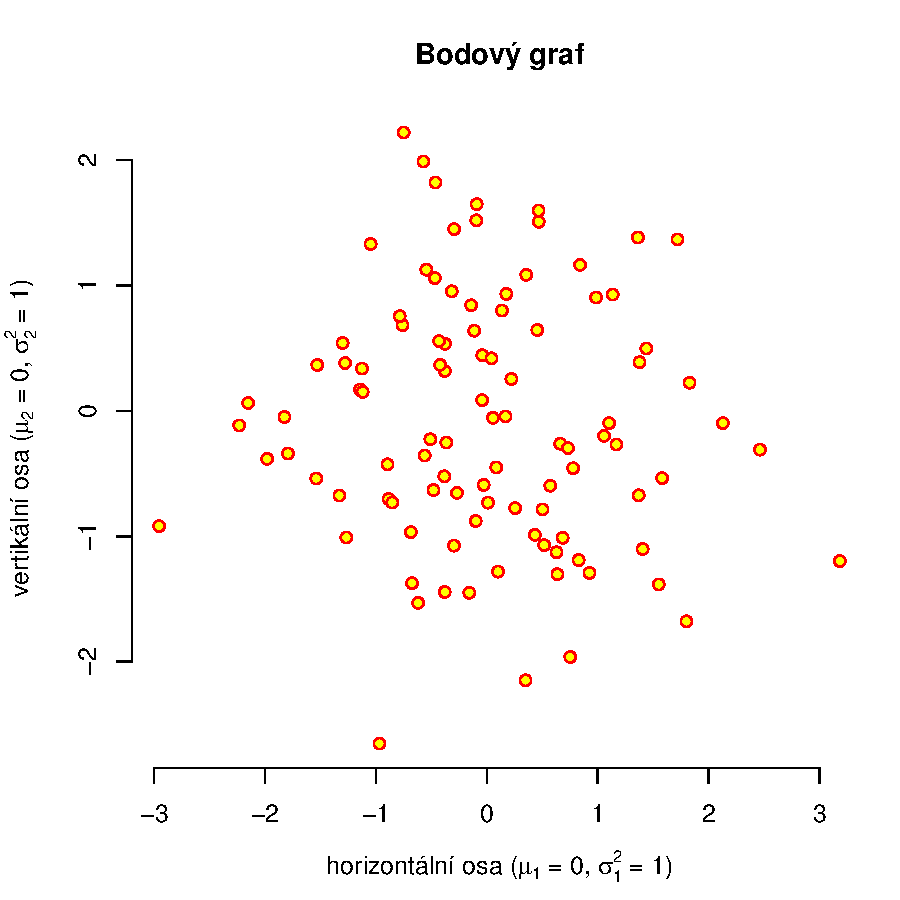
\includegraphics[width=140mm, height=140mm]{../img/ukazka-obr01}
% Příponu není potřeba explicitně uvádět, pdflatex automaticky hledá pdf.
% Rozměry také není nutné uvádět.
\caption{Náhodný výběr z~rozdělení $\mathcal{N}_2(\boldsymbol{0},\,I)$.}
\label{obr03:Nvyber}

\end{figure}

\begin{figure}[p]\centering
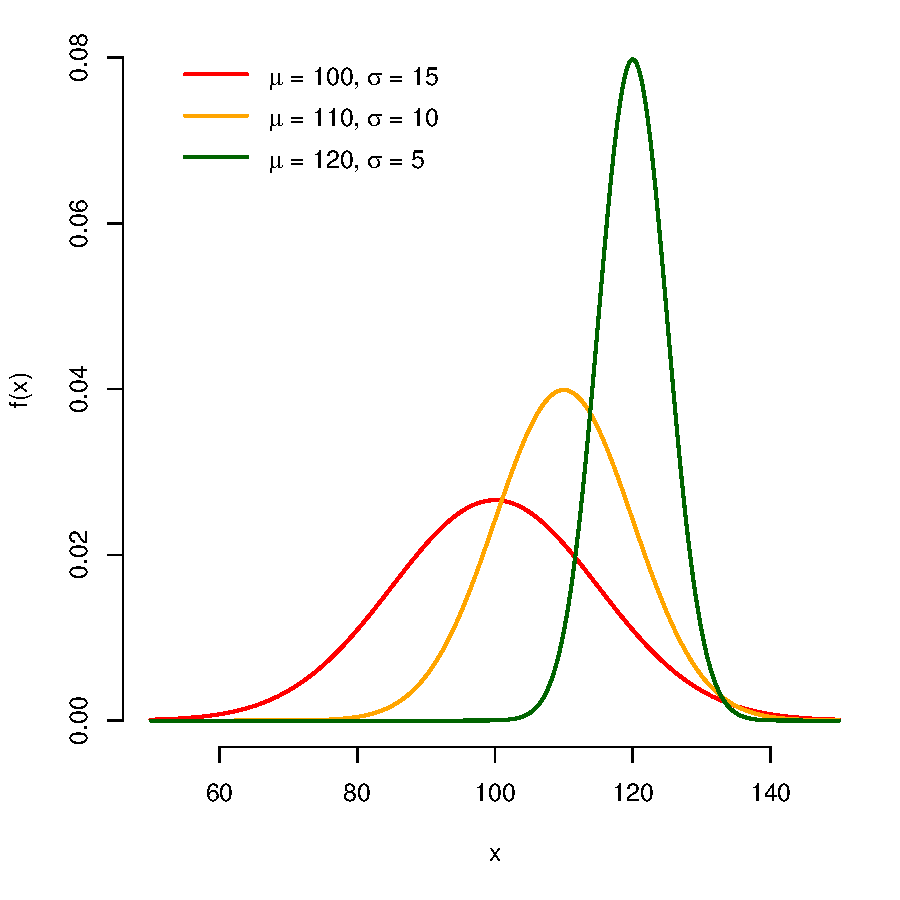
\includegraphics[width=140mm, height=140mm]{../img/ukazka-obr02}
\caption{Hustoty několika normálních rozdělení.}
\label{obr03:Nhust}
\end{figure}

\begin{figure}[p]\centering
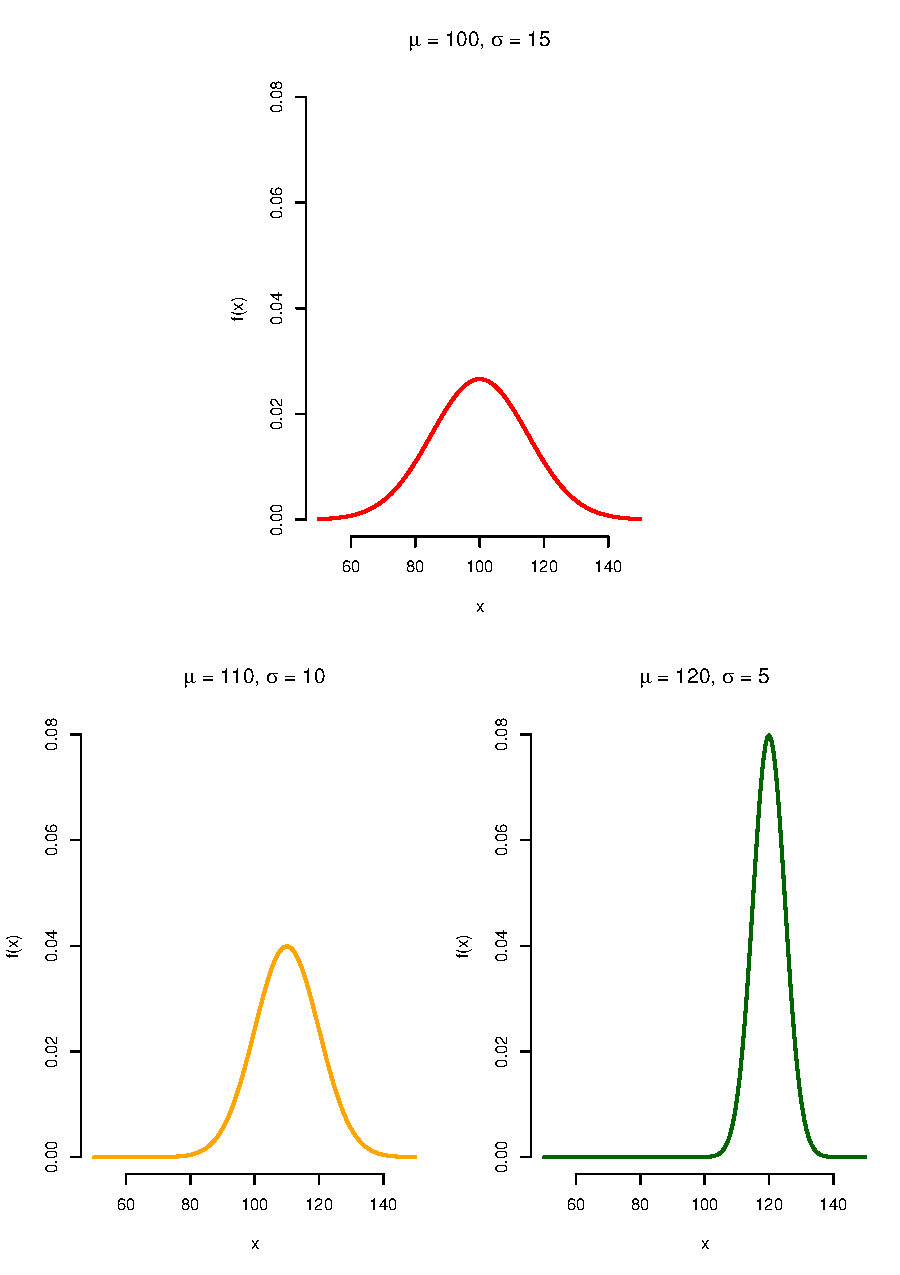
\includegraphics[width=140mm, height=198mm]{../img/ukazka-obr03}
\caption{Hustoty několika normálních rozdělení.}
\label{obr03:Nhust:podruhe}

\end{figure}

%	%%% Fiktivní kapitola s instrukcemi k PDF/A

\chapter{Formát PDF/A}

Opatření rektora č. 13/2017 určuje, že elektronická podoba závěrečných
prací musí být odevzdávána ve formátu PDF/A úrovně 1a nebo 2u. To jsou
profily formátu PDF určující, jaké vlastnosti PDF je povoleno používat,
aby byly dokumenty vhodné k~dlouhodobé archivaci a dalšímu automatickému
zpracování. Dále se budeme zabývat úrovní 2u, kterou sázíme \TeX{}em.

Mezi nejdůležitější požadavky PDF/A-2u patří:

\begin{itemize}

\item Všechny fonty musí být zabudovány uvnitř dokumentu. Nejsou přípustné
odkazy na externí fonty (ani na \uv{systémové}, jako je Helvetica nebo Times).

\item Fonty musí obsahovat tabulku ToUnicode, která definuje převod z~kódování
znaků použitého uvnitř fontu to Unicode. Díky tomu je možné z~dokumentu
spolehlivě extrahovat text.

\item Dokument musí obsahovat metadata ve formátu XMP a je-li barevný,
pak také formální specifikaci barevného prostoru.

\end{itemize}

Tato šablona používá balíček {\tt pdfx,} který umí \LaTeX{} nastavit tak,
aby požadavky PDF/A splňoval. Metadata v~XMP se generují automaticky podle
informací v~souboru {\tt prace.xmpdata} (na vygenerovaný soubor se můžete
podívat v~{\tt pdfa.xmpi}).

Validitu PDF/A můžete zkontrolovat pomocí nástroje VeraPDF, který je
k~dispozici na \url{http://verapdf.org/}.

Pokud soubor nebude validní, mezi obvyklé příčiny patří používání méně
obvyklých fontů (které se vkládají pouze v~bitmapové podobě a/nebo bez
unicodových tabulek) a vkládání obrázků v~PDF, které samy o~sobě standard
PDF/A nesplňují.

Další postřehy o~práci s~PDF/A najdete na \url{http://mj.ucw.cz/vyuka/bc/pdfaq.html}.


	\chapter*{Závěr}
\addcontentsline{toc}{chapter}{Závěr}


%%% Seznam použité literatury
	%%% Seznam použité literatury (bibliografie)
%%%
%%% Pro vytváření bibliografie používáme bibTeX. Ten zpracovává
%%% citace v textu (např. makro \cite{...}) a vyhledává k nim literaturu
%%% v souboru literatura.bib.
%%%
%%% Příkaz \bibliographystyle určuje, jakým stylem budou citovány odkazy
%%% v textu. V závorce je název zvoleného souboru .bst. Styly plainnat
%%% a unsrt jsou standardní součástí latexových distribucí. Styl czplainnat
%%% je dodáván s touto šablonou a bibTeX ho hledá v aktuálním adresáři.

\bibliographystyle{czplainnat}    %% Autor (rok) s českými spojkami
% \bibliographystyle{plainnat}    %% Autor (rok) s anglickými spojkami
% \bibliographystyle{unsrt}       %% [číslo]

\renewcommand{\bibname}{Seznam použité literatury}

%%% Vytvoření seznamu literatury. Pozor, pokud jste necitovali ani jednu
%%% položku, seznam se automaticky vynechá.

\bibliography{literatura}

%%% Kdybyste chtěli bibliografii vytvářet ručně (bez bibTeXu), lze to udělat
%%% následovně. V takovém případě se řiďte normou ISO 690 a zvyklostmi v oboru.

% \begin{thebibliography}{99}
%
% \bibitem{lamport94}
%   {\sc Lamport,} Leslie.
%   \emph{\LaTeX: A Document Preparation System}.
%   2. vydání.
%   Massachusetts: Addison Wesley, 1994.
%   ISBN 0-201-52983-1.
%
% \end{thebibliography}


%%% Obrázky v bakalářské práci
%%% (pokud jich je malé množství, obvykle není třeba seznam uvádět)
	\listoffigures

%%% Tabulky v bakalářské práci (opět nemusí být nutné uvádět)
%%% U matematických prací může být lepší přemístit seznam tabulek na začátek práce.
	\listoftables

%%% Použité zkratky v bakalářské práci (opět nemusí být nutné uvádět)
%%% U matematických prací může být lepší přemístit seznam zkratek na začátek práce.
	\chapwithtoc{Seznam použitých zkratek}

%%% Přílohy k bakalářské práci, existují-li. Každá příloha musí být alespoň jednou
%%% odkazována z vlastního textu práce. Přílohy se číslují.
%%%
%%% Do tištěné verze se spíše hodí přílohy, které lze číst a prohlížet (dodatečné
%%% tabulky a grafy, různé textové doplňky, ukázky výstupů z počítačových programů,
%%% apod.). Do elektronické verze se hodí přílohy, které budou spíše používány
%%% v elektronické podobě než čteny (zdrojové kódy programů, datové soubory,
%%% interaktivní grafy apod.). Elektronické přílohy se nahrávají do SISu a lze
%%% je také do práce vložit na CD/DVD. Povolené formáty souborů specifikuje
%%% opatření rektora č. 72/2017.
	\appendix


	\chapter{Přílohy}


	\section{První příloha}

	\openright
\end{document}
